\documentclass[a4paper,12pt,oneside]{book}

%-------------------------------Start of the Preable------------------------------------------------
\usepackage[english]{babel}
\usepackage[utf8]{inputenc}
\usepackage{blindtext}
%packagr for hyperlinks
\usepackage{hyperref}
\hypersetup{
    colorlinks=true,
    linkcolor=blue,
    filecolor=magenta,      
    urlcolor=cyan,
}

\urlstyle{same}
%use of package fancy header
\usepackage[toc,page]{appendix}
\usepackage{fancyhdr}
\usepackage{float}
\usepackage{subfig}
\setlength\headheight{26pt}
\fancyhf{}
%\rhead{
\includegraphics[width=1cm]{logo}}
\lhead{\rightmark}
\rhead{
\includegraphics[width=1cm]{logo}}
\fancyfoot[RE, RO]{\thepage}
\fancyfoot[CE, CO]{\href{http://www.e-yantra.org}{www.e-yantra.org}}

\pagestyle{fancy}

%use of package for section title formatting
\usepackage{titlesec}
\titleformat{\chapter}
  {\Large\bfseries} % format
  {}                % label
  {0pt}             % sep
  {\huge}           % before-code
 
%use of package tcolorbox for colorful textbox
\usepackage[most]{tcolorbox}
\tcbset{colback=cyan!5!white,colframe=cyan!75!black,halign title = flush center}

\newtcolorbox{mybox}[1]{colback=cyan!5!white,
colframe=cyan!75!black,fonttitle=\bfseries,
title=\textbf{\Large{#1}}}

%use of package marginnote for notes in margin
\usepackage{marginnote}

%use of packgage watermark for pages
%\usepackage{draftwatermark}
%\SetWatermarkText{
\includegraphics{logo}}
\usepackage[scale=2,opacity=0.1,angle=0]{background}
\backgroundsetup{
contents={
\includegraphics{logo}}
}

%use of newcommand for keywords color
\usepackage{xcolor}
\newcommand{\keyword}[1]{\textcolor{red}{\textbf{#1}}}

%package for inserting pictures
\usepackage{graphicx}

%package for highlighting
\usepackage{color,soul}

%new command for table
\newcommand{\head}[1]{\textnormal{\textbf{#1}}}
\graphicspath{ {images/} } 

%----------------------End of the Preamble---------------------------------------


\begin{document}

%---------------------Title Page------------------------------------------------
\begin{titlepage}
	\raggedright
	{\Large eYSIP2016\\[1cm]}
	{\Large\scshape GREENHOUSE POWER MONITORING AND APPLIANCE CONTROL \\[.1in]}
	
	\vfill
	
	{\underline{\large{Interns:}}} \\
	\begin{quote}
		\large{Avilash Mohanty}
		
		\large{Email: avilashmohanty1920@gmail.com}		
		
		\large{Mobile: 9560372680}
	\end{quote}
	
	
	
	\begin{quote}
		\large{Abhishek Acharya}
		
		\large{Email: abhi11796acharaya@gmail.com}	
		
		\large{Mobile: 8014692750}
	\end{quote}
	
	
	\vspace{0.5cm}
	
	{\underline{\textbf{Mentors:}}} \\
	\begin{quote}
		\large{Saurav Shandilya}\\
		\large{Vishwanathan Iyer}\\
		\large{Parin Chheda}\\
	
		
	\end{quote}
	
	
	
	\begin{flushright}
		{\large Duration of Internship: $ 10/06/2016-24/07/2016 $ \\}
		
	\end{flushright}
	{\itshape 2016, e-Yantra Publication}
	
	
	
\end{titlepage}
%-------------------------------------------------------------------------------

\tableofcontents
%-------------------------------------------------------------------------------
\chapter[Greenhouse Power Monitoring and Appliance Control]{Greenhouse Power Monitoring and Appliance Control }
\section{Abstract}
\hspace{7mm}This project aims at developing a monitoring system which will consist of a Wi-Fi enabled device which can measure the basic electrical paramenters of greenhouse's electrical appliances. This system will have Web based GUI through which user can monitor real-time graphically visualised data. 
The monitored parameters will be logged in a database for future reference and  plotted on the web GUI logging page. This Web GUI also enables the user to switch and schedule ON/OFF time of the device as per requirement.
\\

\newpage

\section{Completion status}
\begin{itemize}
	\item{Tasks Accomplished}
	\setlength\itemsep{0.2cm}
	\begin{enumerate}
		\item{Literature survey of existing Real time Web Monitoring sites. }    
		\item{Developed a Circuit to measure Current,Voltage,Phase and Frequency.}
		\item{Research and finalisation on Micro-controller board and Softwares to be used.}
		\item{Measurement of Current,Voltage,Phase and Frequency.}
		\item{Established a connection between server and micro-controller.}
		\item{Logged Real time data in database.}
		\item{Created Real Time updating Charts.}
		\item{Graphical Visualisation of logged data.}
		\item{Interfaced relay with the micro-controller.}
		\item{Created a Webpage to control the connected devices.}
		\item{Scheduling on/off time of devices.}
		\item{3 device support for monitoring and controlling.}
		\item{Feedback system to compare real-device status and system's  data.}
		\item{Terminal based GUI to configure the 'Smart Switchboard/Plug'.}
		\item{Code Documentation and Project Report.}
	\end{enumerate}
	\item{Incomplete Tasks}
	\begin{enumerate}
		\item{Responsive web design. }
	\end{enumerate}
	\par Front-end can be improved and made responsive by using bootstrap.   
\end{itemize}

\newpage
\section{Hardware parts}
\begin{enumerate}
  \item \textbf{List of hardware used:-}\\
  
		 \begin{tabular}{|l|c|c|}
		 	\hline
		 	\textbf{Name of hardware} & \textbf{Specification} & \textbf{Quantity} \\ \hline
		 	Electrical Switch Board& 2-Plug and 1 Bulb Holder & 1\\ 
		 	& and 3 switches&\\\hline
		 	Potential Transformer& 230V-9V 100mA &1 \\ \hline
		 	Hall Effect Sensor Module& ACS712 (30A) &3\\ \hline
		 	Bulb& 100W & 1\\ \hline
		 	& TI's CC3200-LAUNCHXL&\\
		 	CC3200-LAUNCHPAD&\textit{(With CC3200-HZ on } &1 \\
		 	&\textit{ chip wifi microcontroller)} &\\\hline
		 	Soldring Iron& 220V, 40W &1 \\ \hline
		 	Soldring Wire& 50gm & 1 \\ \hline
		 	Jumper Wires& Female to Female & \\\cline{2-3}
		 	&Male to Female& \\\hline
		 	4-Channel Relay Board& 230V AC (10Amp)& 1\\ \hline
		 	Measurement Board& & \\ 
		 	\textit{(Designed \& Developed } & MBV1.1 & 1 \\
		 	\textit{ \hspace{1cm} during eYSIP-16) } & & \\ \hline
		 \end{tabular}
		 \vspace{1cm}
	\item \textbf{Details of hardware used:-}
	\begin{itemize}
		  \item Electrical Switch Board (Purchased from local market) 
		  \item Potential Transformer\href{http://www.industrybuying.com/transformer-transformers-EL.TR1.380140/?utm_source=Google&utm_medium=PLA&utm_campaign=0_PLA_HPP&gclid=Cj0KEQjw_eu8BRDC-YLHusmTmMEBEiQArW6c-KfZiqs2kmbBI3vn0sM1cPt5KuvFcSrQhloBs1NVNrYaAr428P8HAQ}{Vendor link} 
		  \item Hall Effect Sensor Module \href{https://github.com/eYSIP-2016/eYSIP2016-GHPowerMonitoring/blob/master/Documents/report_eYSIP_GHpowerMonitoring/datasheet/ACS712-Datasheet.pdf}{Datasheet},\href{http://www.amazon.in/Current-Sensor-Module-ACS712-model/dp/B00NU8XD80?tag=googinhydr18418-21&tag=googinkenshoo-21&ascsubtag=8a34ff38-5122-429d-8260-7633d5ca1fcf}{Vendor link},
		  \item Bulb   (Purchased from local market) 
		  \item CC3200 LAUNCHPAD \href{./datasheet/cc3200 complete datasheet.pdf}{Datasheet}, 		\href{https://www.fabtolab.com/boards/TI}{Vendor link}
		  \item Jumper Wires  \href{https://www.fabtolab.com}{Vendor link}
		  \item 4-Channel Relay Board \href{./datasheet/relay.pdf}{Datasheet}, \href{http://www.amazon.in/Isolated-Optocoupler-Driver-Expansion-Module/dp/B00NR31V3W?tag=googinhydr18418-21&tag=googinkenshoo-21&ascsubtag=8a34ff38-5122-429d-8260-7633d5ca1fcf}{Vendor link}
		  \item Measurement Board for manual refer section \autoref{100} of appendix.
	\end{itemize}
	\newpage
  \item \textbf{Connection diagram:-}
  \begin{figure}[h]
  	\includegraphics[width=390px]{connection}
  \end{figure}
  \\\textbf{HERE:-} 
   \begin{itemize}
   	\item A1:  current sensor input pin 1 (Analog pin)
   	\item A2:  current sensor input pin 2 (Analog pin)
   	\item A3:  current sensor input pin 3 (Analog pin)
   	\item V1:  transformer output pin (Analog pin)
   	\item C1:  current1 signal out pin (Analog pin)
   	\item C2:  current2 signal out pin (Analog pin)
   	\item V1:  voltage signal out pin (Analog pin)
   	\item F1:  frequency signal out pin (Digital pin)
   	\item PH1:  phase 1 signal out pin (Digital pin)
   	\item PH2:  phase 2 signal out pin (Digital pin)
   	\item All the pins used in CC3200 Launchpad are General purpose I/O pins.
   \end{itemize}
\end{enumerate}

\newpage
\section{Software used}
\begin{enumerate}
	\item\textbf{ Code Composer Studio} \\
  -- Detail of software: version 6.1.3.00033, \href{http://www.ti.com}{download link}\\
  -- Installation steps:
  \begin{itemize}
  	\item click on the rar file named $"CCS6.1.3.00033\_win32"$
  	  \begin{figure}[h]
  	  	\hspace{2cm}
  	 	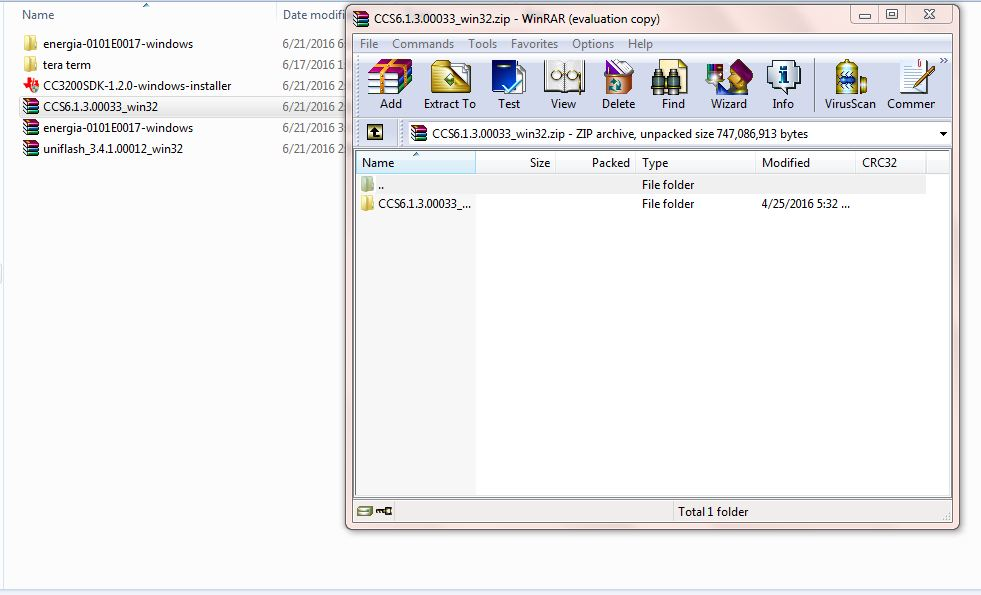
\includegraphics[width=300px]{inst1}
  	 \end{figure}
  	 	 \item Now click on the extracted folder
  	  \begin{figure}[h]
  	  		\hspace{2cm}
  	 	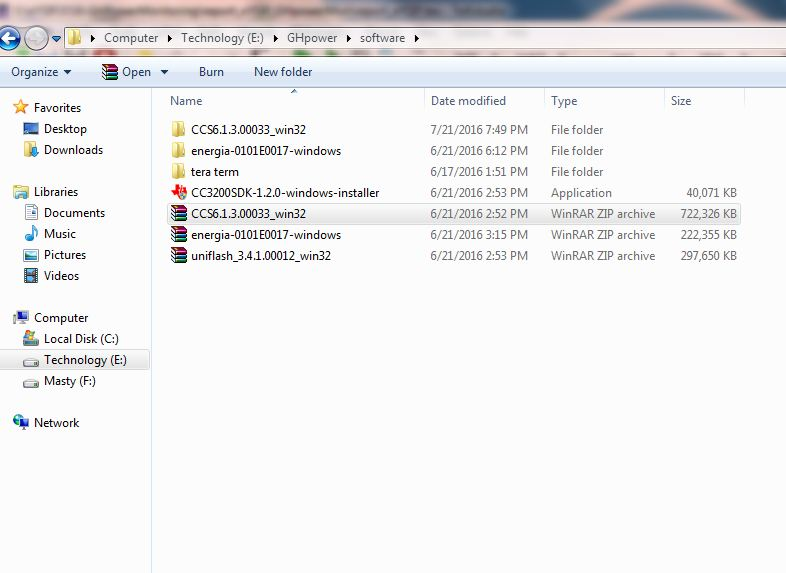
\includegraphics[width=300px]{inst2}
  	 \end{figure}
  	 \newpage
  	 \item click on the .exe setup file
  	 \begin{figure}[h]
  	 		\hspace{2cm}
  	  	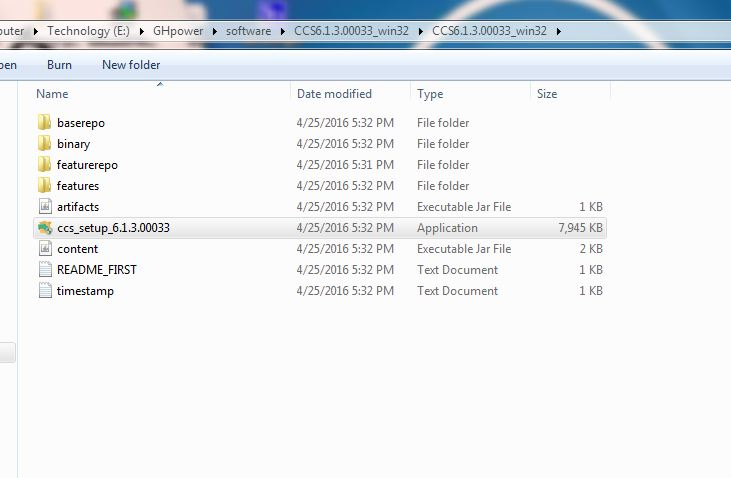
\includegraphics[width=300px]{inst3}
  	 \end{figure}
  	 \item Accept License agreement and click on next to complete the installation of Code Composer Studio.
  	 \begin{figure}[h]
  	 		\hspace{2cm}
  	 	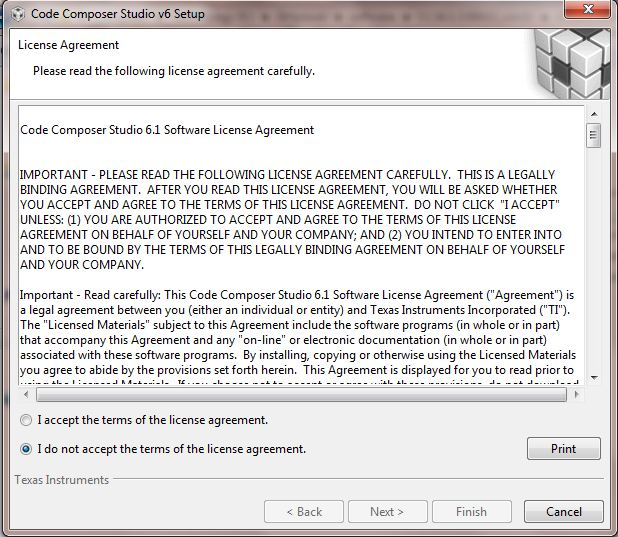
\includegraphics[width=250px]{inst4}
  	  \end{figure} 
  	  \newpage
  	  \item \textbf{Energia}
  	   -- Detail of software: version 6.1.3.00033, \href{http://www.energia.nu}{download link}\\
  	   -- Installation steps:
  	   \begin{itemize}
  	   	\item click on the rar file named $"energia-0101E0017-windows"$
  	   	\begin{figure}[h]
  	   		\hspace{2cm}
  	   		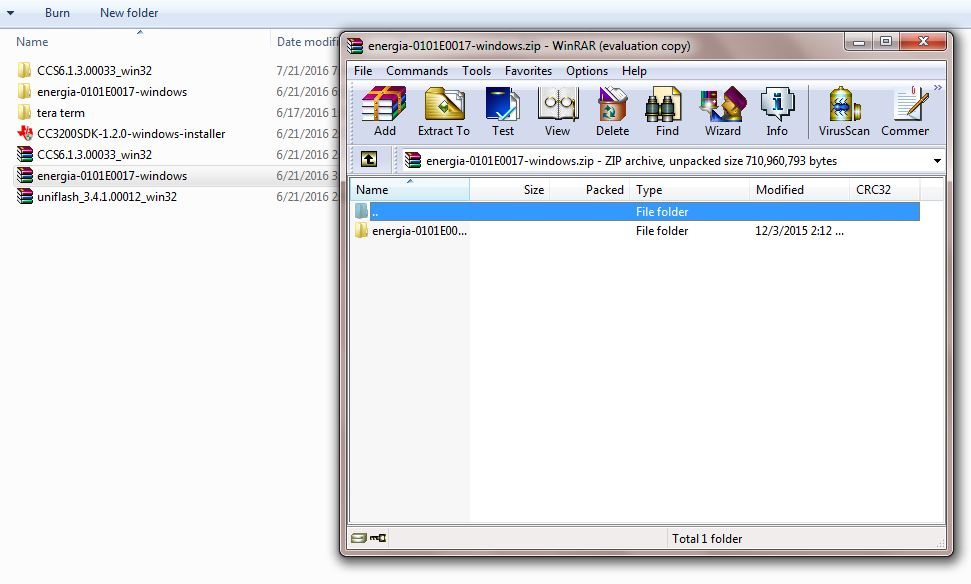
\includegraphics[width=300px]{inst5}
  	   	\end{figure}
  	   \end{itemize}
  	   \item Now click on extracted folder with same name
  	   \begin{figure}[h]
  	   	\hspace{2cm}
  	   	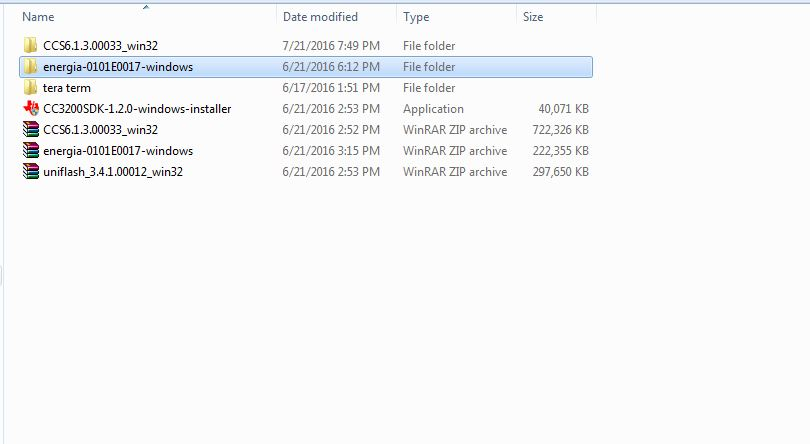
\includegraphics[width=300px]{inst6}
  	   \end{figure}
  	     \newpage
  	   \item click on energia .exe application file
  	   \begin{figure}[h]
  	   	\hspace{2cm}
  	   	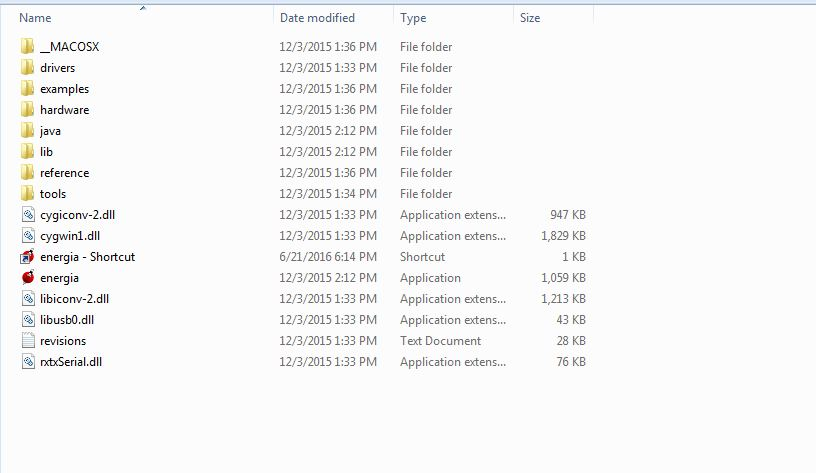
\includegraphics[width=300px]{inst7}
  	   \end{figure}
  	   \item code compile upload and enjoy
  	   \begin{figure}[h]
  	   	\hspace{2cm}
  	   	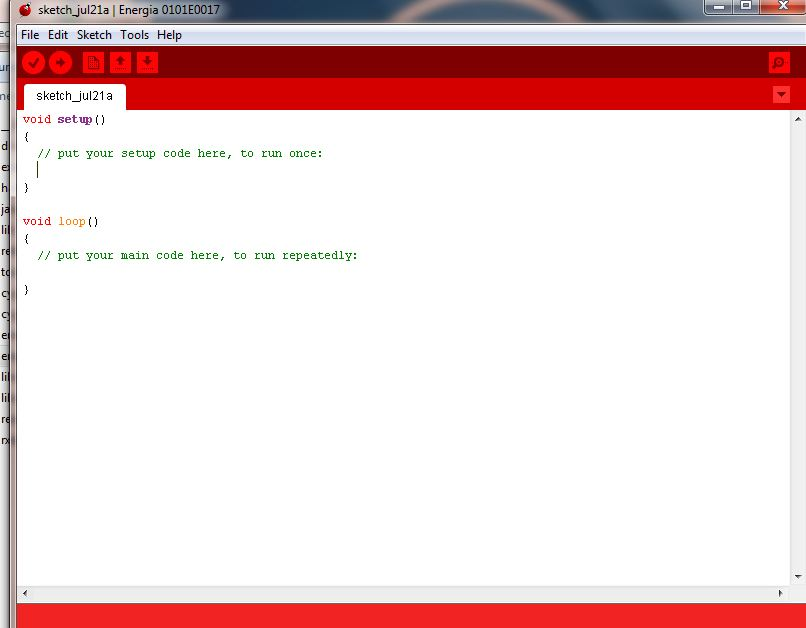
\includegraphics[width=300px]{inst8}
  	   \end{figure}
  \end{itemize}
  \newpage
  	\item\textbf{CCS Uniflash} \\
  	-- Detail of software: version 3.4, \href{http://www.ti.com}{download link}\\
  	-- Installation steps:
    \begin{itemize}
    	\item click on the rar file named $"uniflash\_3.4.1.00012\_win32"$
    	\begin{figure}[h]
    		\hspace{2cm}
    		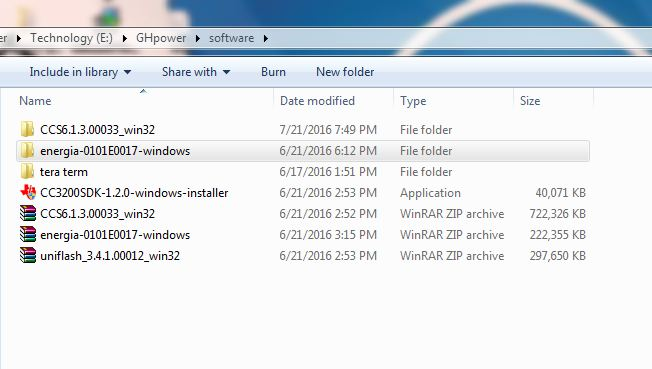
\includegraphics[width=300px]{inst9}
    	\end{figure}
    \item Now click on extracted folder with same name
    \begin{figure}[h]
    	\hspace{2cm}
    	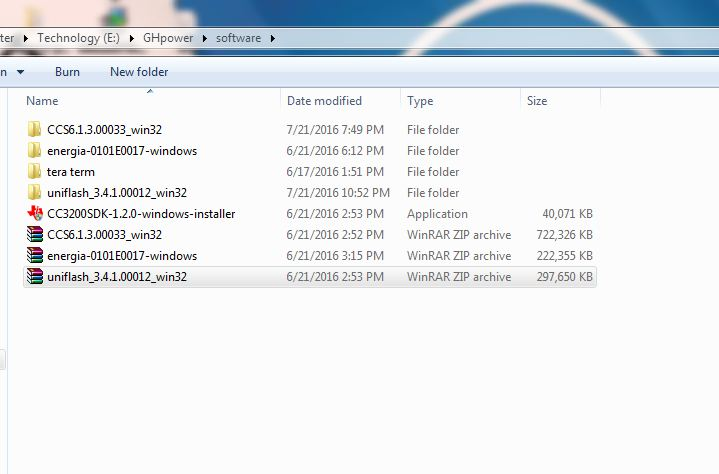
\includegraphics[width=300px]{inst10}
    \end{figure}
    \newpage
    \item click on $uniflash\_win.exe$ application file and continue to click on next till installation complete.
    \begin{figure}[h]
    	\hspace{2cm}
    	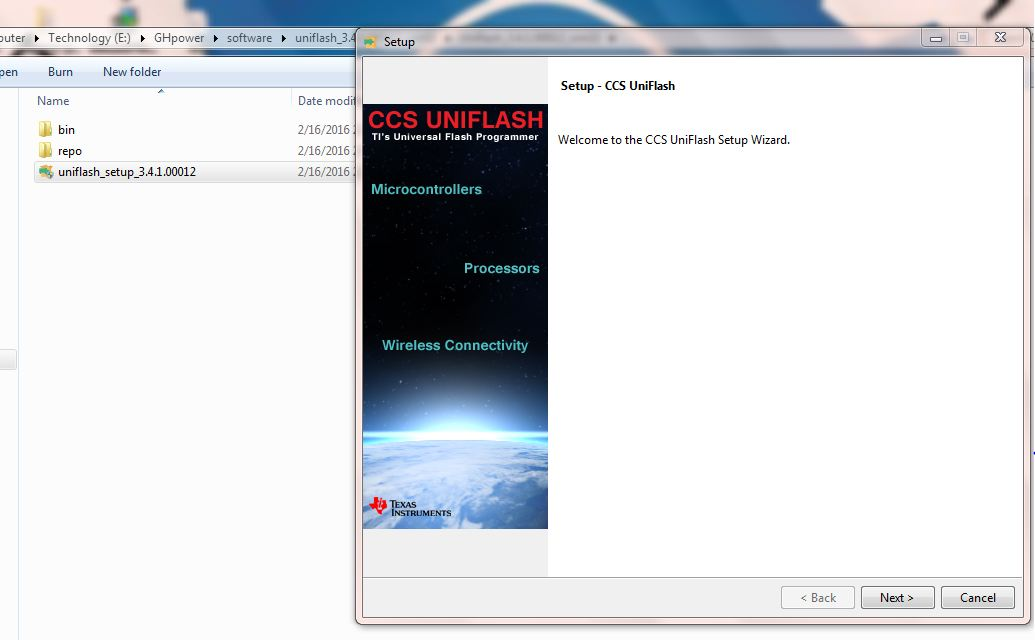
\includegraphics[width=300px]{inst11}
    \end{figure}
    \begin{figure}[h]
    	\hspace{2cm}
    	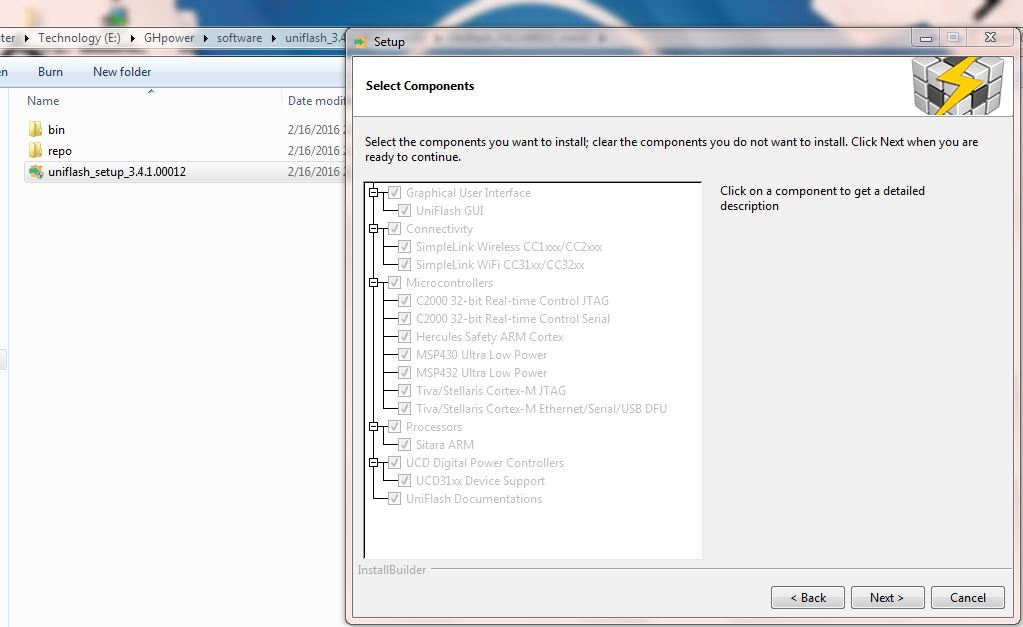
\includegraphics[width=300px]{inst12}
    \end{figure}
    \newpage
     \item open uniflash, select COM port and make a .ccxml file for cc3200 launchpad
     \begin{figure}[h]
     	\hspace{2cm}
     	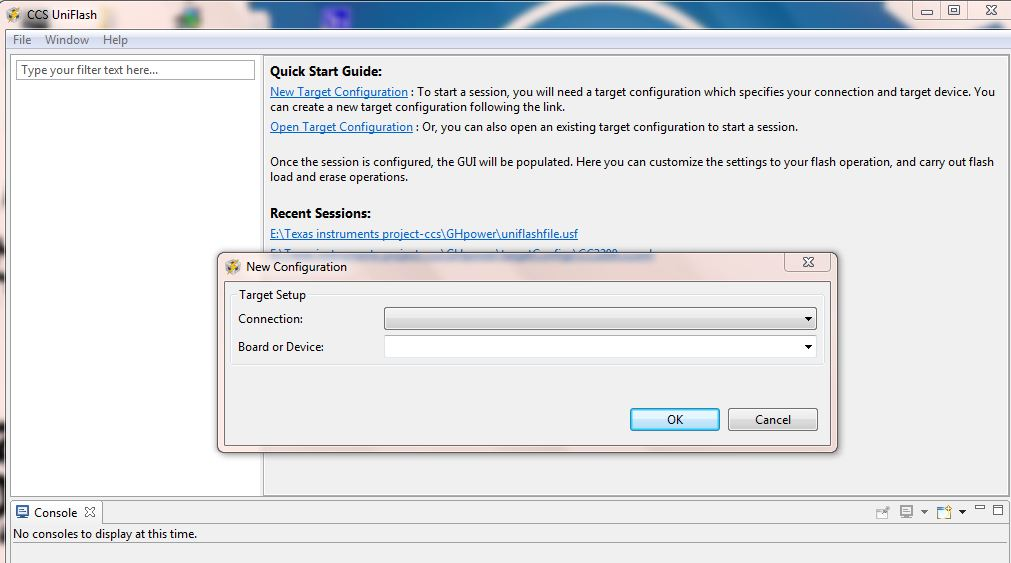
\includegraphics[width=300px]{inst13}
     \end{figure}
\end{itemize}
\newpage
	\item\textbf{ CC3200 SDK from TI} \\
	-- Detail of software: version 1.2.0, \href{http://www.ti.com}{download link}\\
	-- Installation steps:
\begin{itemize}
	 \item click on CC3200SDK.exe application file and install the sdk by clicking next button till installation complete
	 \begin{figure}[h]
	 	\hspace{2cm}
	 	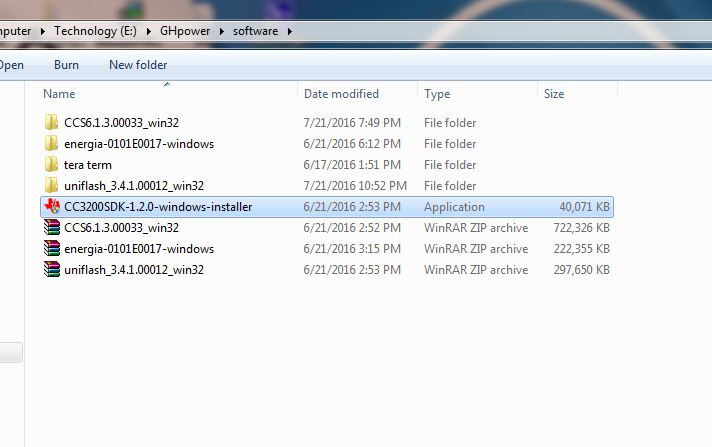
\includegraphics[width=300px]{inst14}
	 \end{figure}
	 \begin{figure}[h]
	 	\hspace{2cm}
	 	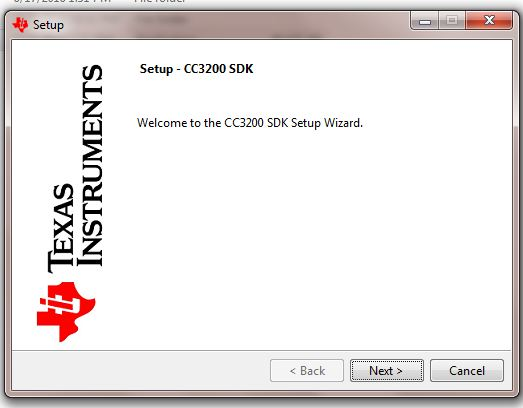
\includegraphics[width=300px]{inst15}
	 \end{figure}
\end{itemize}
\newpage
\item\textbf{ CC3200 service pack} \\
-- Detail of software: version 1.0.0.1.2, \href{http://www.ti.com}{download link}\\
   \textbf{note:- service pack should be compatible with your launchpad version}\\
-- Installation steps:
\begin{itemize}
	\item click on CC3200servicepack.exe application file and install the sdk by clicking next button till installation complete
	\begin{figure}[h]
		\hspace{2cm}
		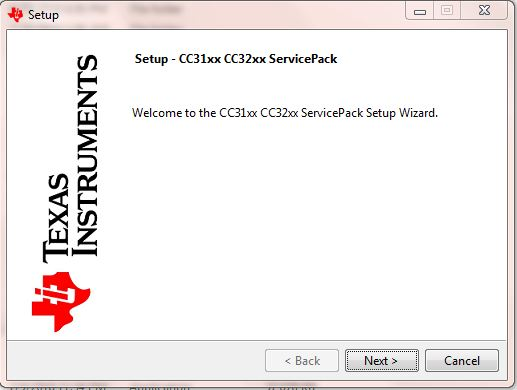
\includegraphics[width=300px]{service1}
	\end{figure}
\end{itemize}
\newpage
\item\textbf{Setting up Serial Terminal software} \\
Serial terminal is used for code debugging and configuring wifi of smart switch board. We have used Coolterm, however any other serial terminal software can be used.  \\
-- Detail of software: version 1.4.6, \href{http://www.coolterm.com}{Coolterm Download Link}\\
	\begin{figure}[h]
		\hspace{2cm}
		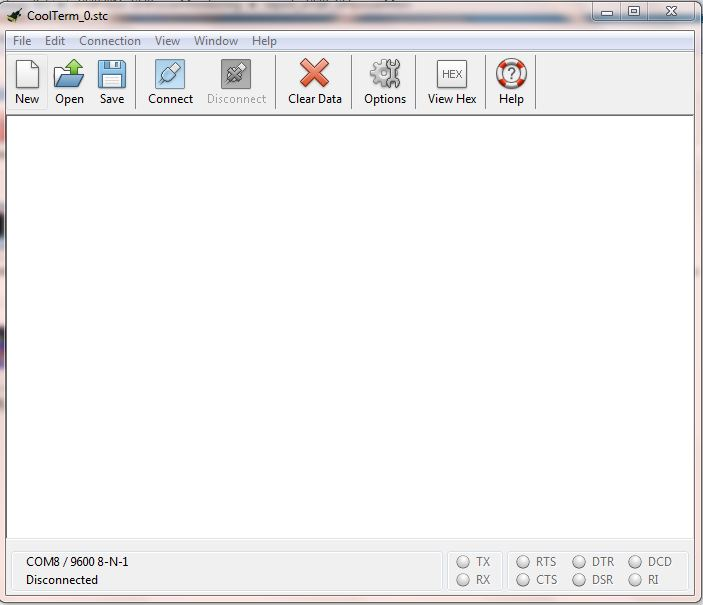
\includegraphics[width=270px]{inst16}
	\end{figure}
%	\begin{figure}[h]
%		\hspace{2cm}
%		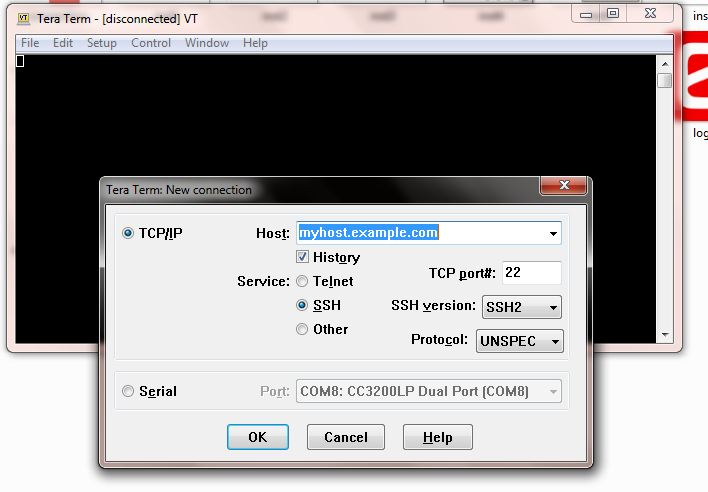
\includegraphics[width=270px]{inst17}
%	\end{figure}
%	\newpage
					\item System Specification
					\begin{enumerate}
						\item Operating System: Windows 10 OS
					\end{enumerate}
					\item Setting up the local Server \& Database
					\begin{enumerate}
						\item Software used: XAMPP
						\item Version: XAMPP version 3.2.2
						\item \href{https://www.apachefriends.org/download.html}{XAMPP Download Link}
						\item \href{http://www.wikihow.com/Install-XAMPP-for-Windows}{XAMPP Installation steps}
						\hspace{20px}
						
%						\begin{figure}[H]  \centering
%							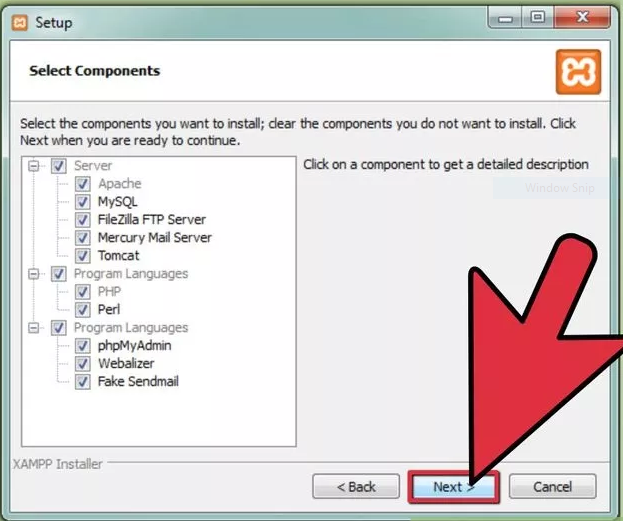
\includegraphics[width=13cm]{xampp1.png}
%							\caption{Component Selection}
%						\end{figure}
%						\begin{figure}[H]  \centering
%							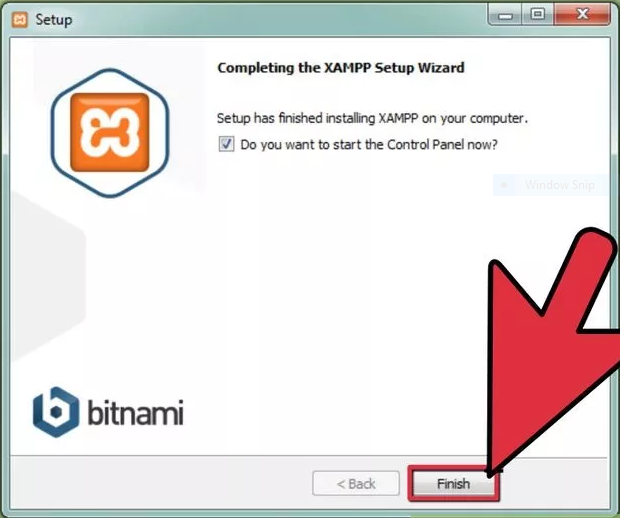
\includegraphics[width=13cm]{xampp12.png}
%							\caption{Finish Installation}
%						\end{figure}
						\begin{figure}[H]  \centering
							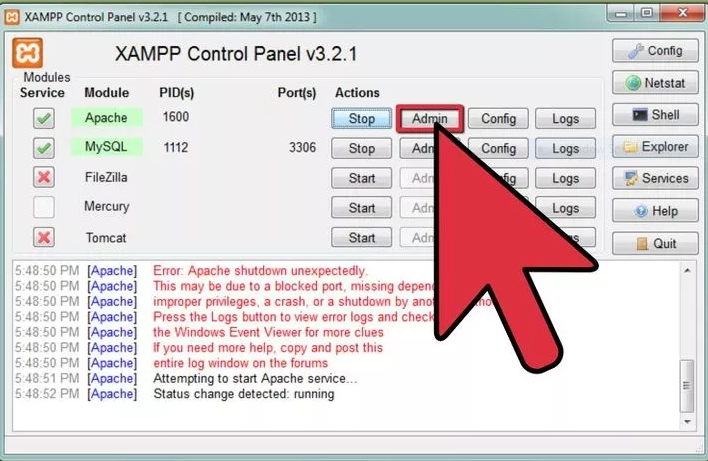
\includegraphics[width=13cm]{xampp3.png}
							\caption{Open XAMPP Control Panel}
						\end{figure}
						%\hspace{10px}
						
						\textbf{NOTE: If Server rejects connection requests by microcontroller, follow these steps.}
						
						\begin{figure}[H]  \centering
							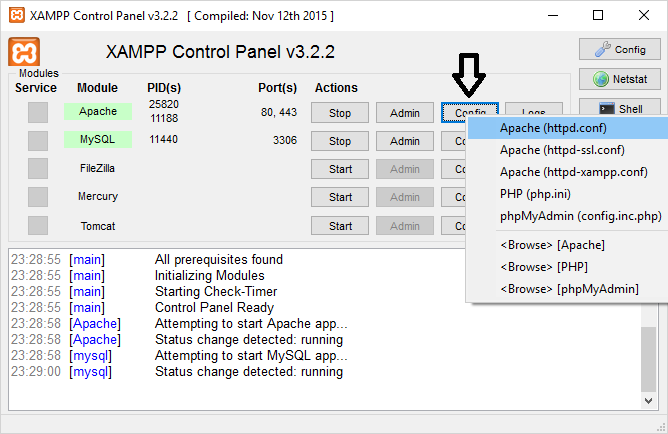
\includegraphics[width=13cm]{httpconf2.png}
							\caption{Open httpd.conf}
							\label{fig:1_Open httpd.conf}
						\end{figure}
						
						\item{Open httpd.conf file in configuration setting for Apache Server in XAMPP, as shown in \ref{fig:1_Open httpd.conf}}
						\begin{figure}[H]  \centering
							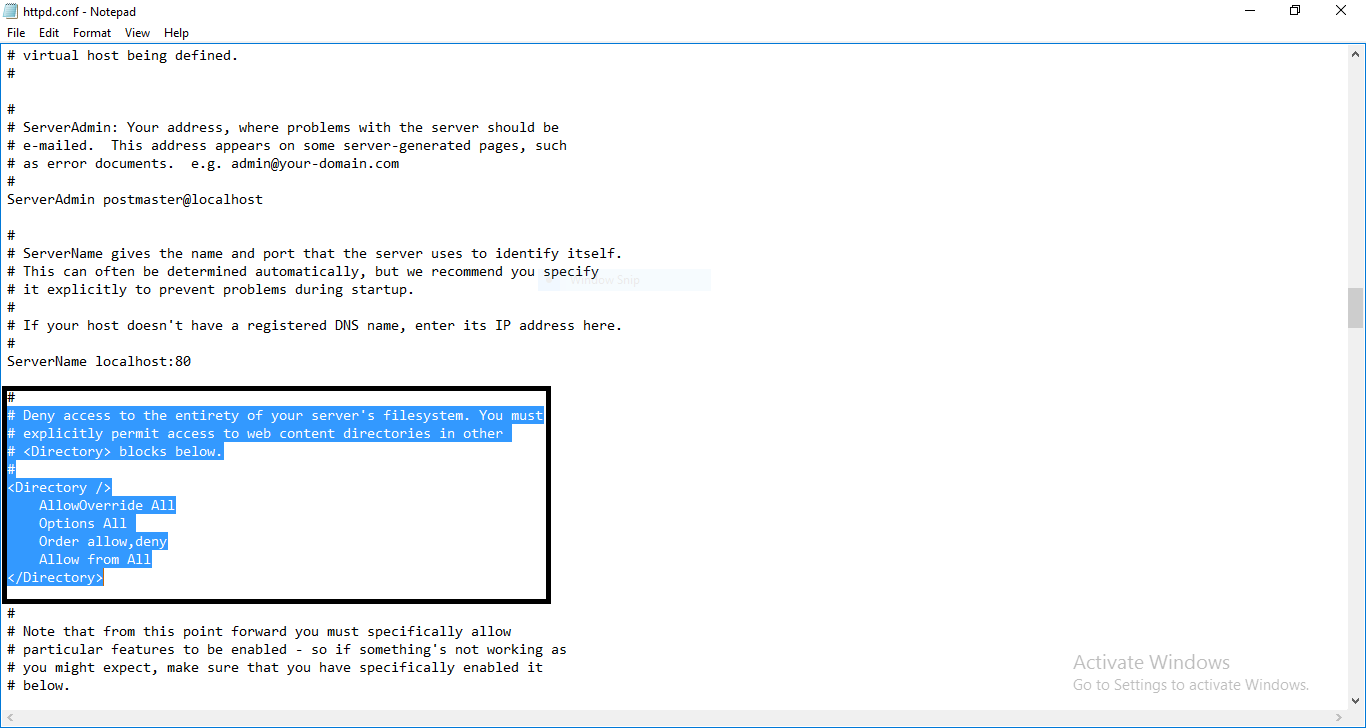
\includegraphics[width=13cm]{override.png}
							\caption{Change httpd.conf}
							\label{fig-2_change httpd.conf}
						\end{figure}
						
						\item{Refer figure \ref{fig-2_change httpd.conf}Set \\ $AllowOverride  All$\\
							$Options All$ \\
							$Order allow,deny$\\
							$Allow from All$ }
						
						
					\end{enumerate}
					\item Setting up the Editor
					\begin{enumerate}
						
						\item Software used : \href{https://notepad-plus-plus.org/download/v6.9.2.html}{ Notepad++ v6.9.2 }
					\end{enumerate}			
\end{enumerate}

\newpage
\section{Assembly of hardware}
Circuit diagram and Steps of assembly of hardware with pictures for each step. For Detailed information about $Measurement\ Board$ \autoref{100}
\subsection*{Circuit Diagram}
\begin{figure}[h]
	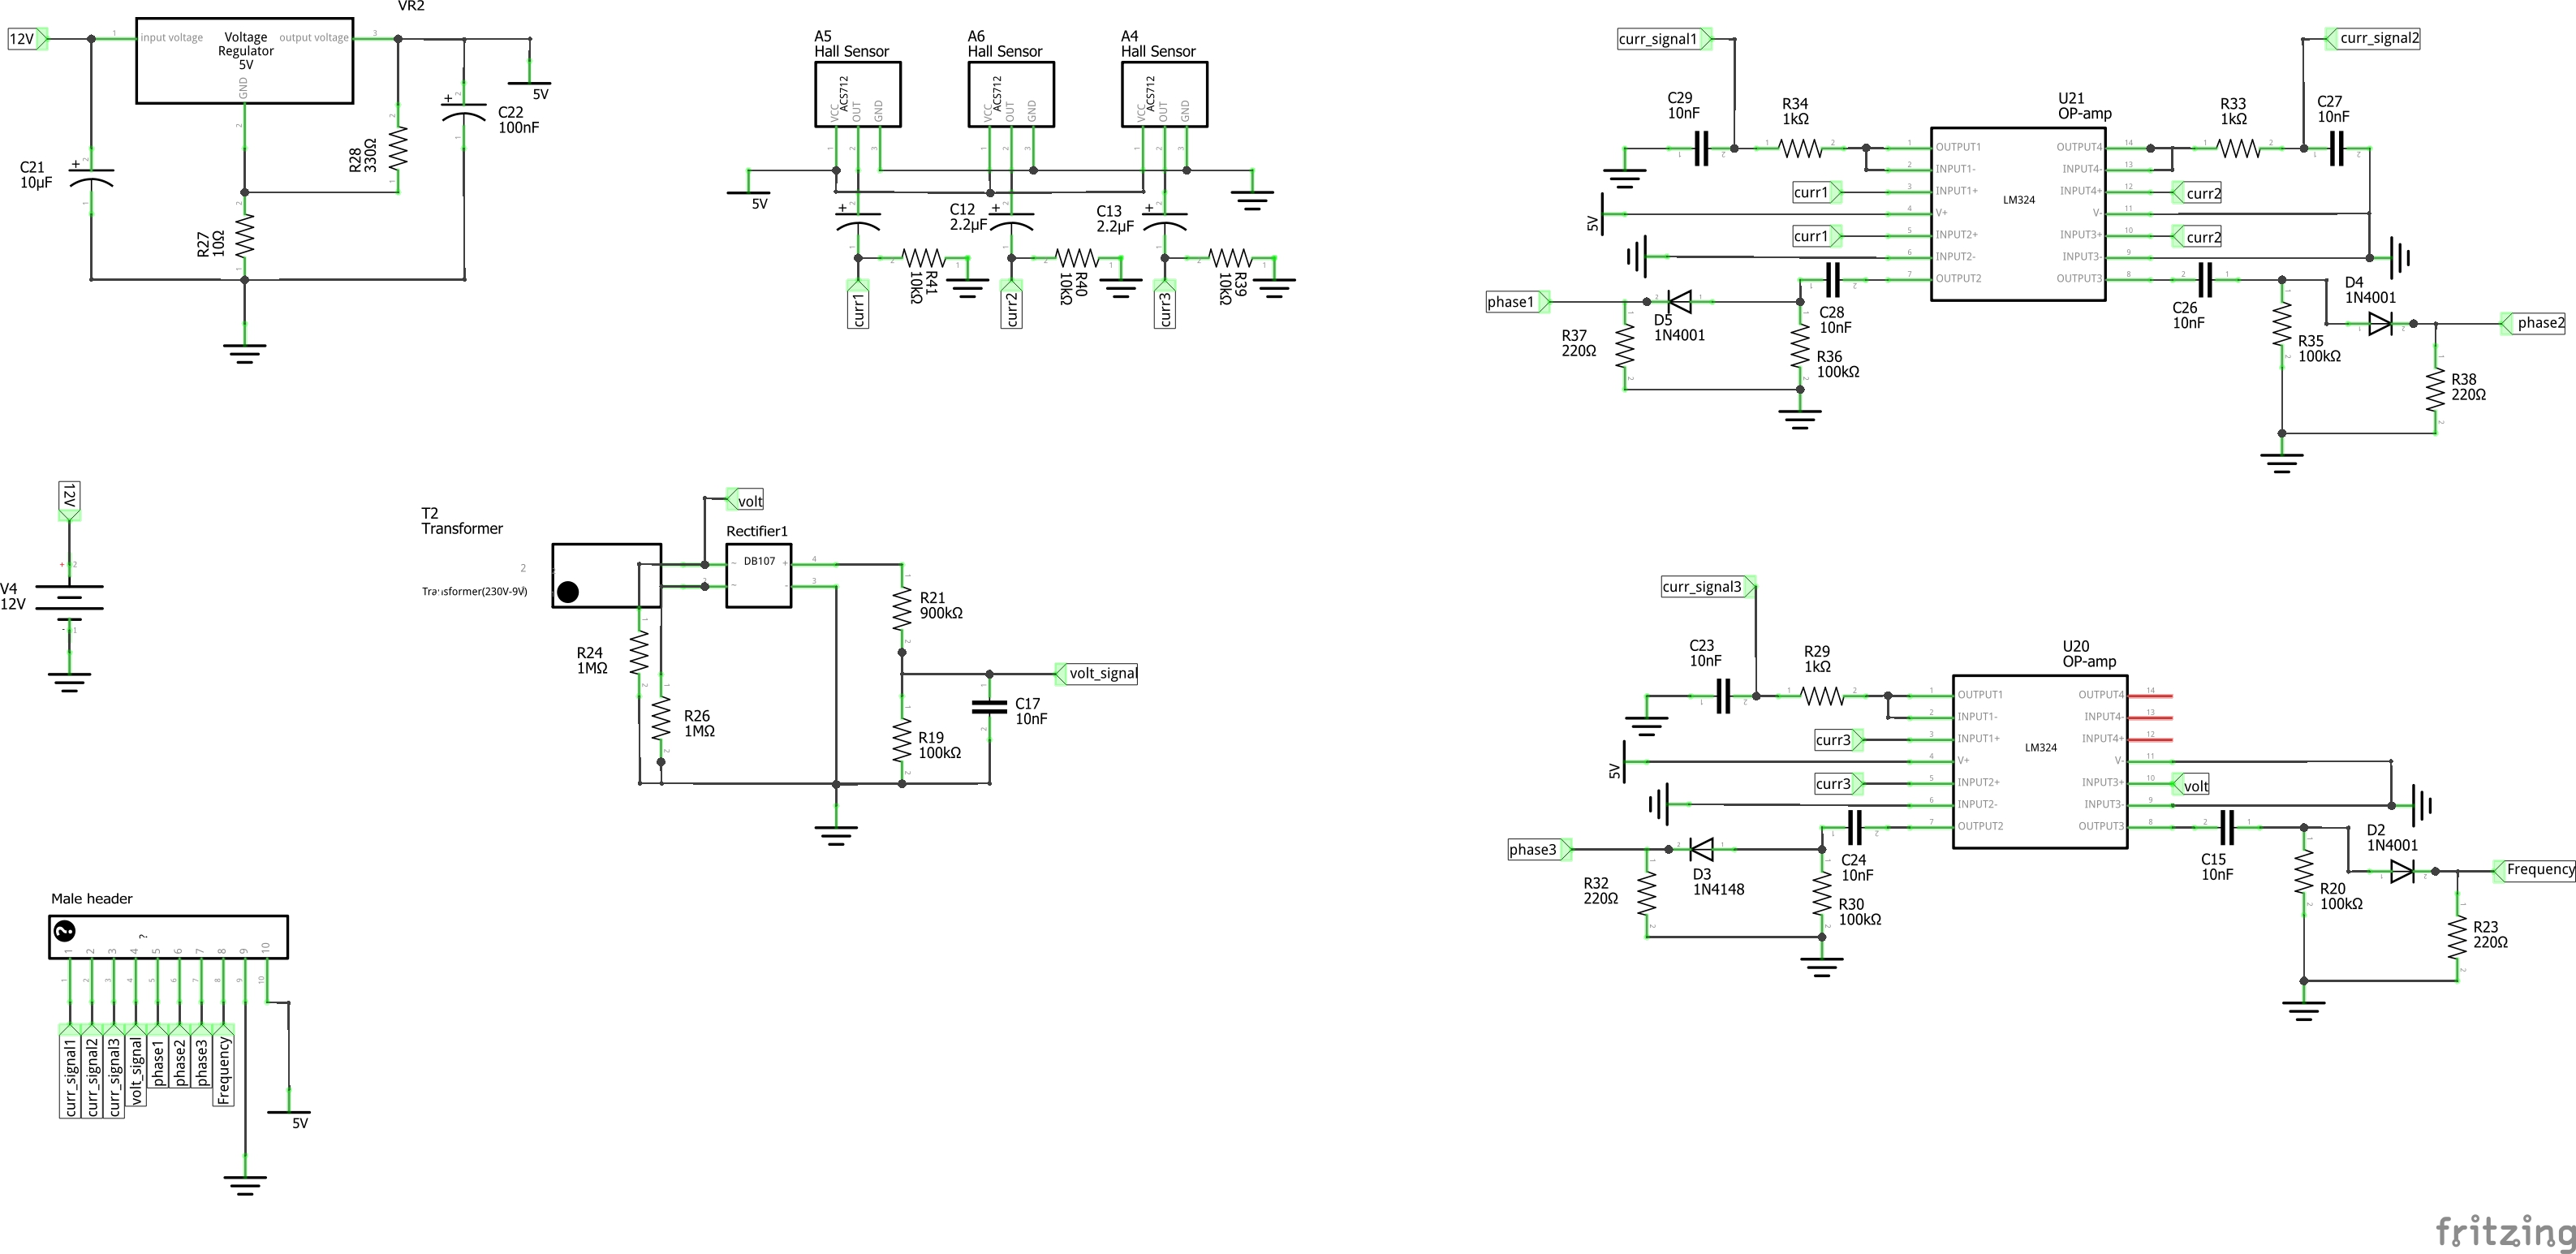
\includegraphics[width=380px,height=380px]{schematic}
\end{figure}
\newpage
\subsection*{Step 1}
Make a basic switch board which has two plug and and one bulb holder mounted on it as 
shown in figure below
\begin{figure}[h]
	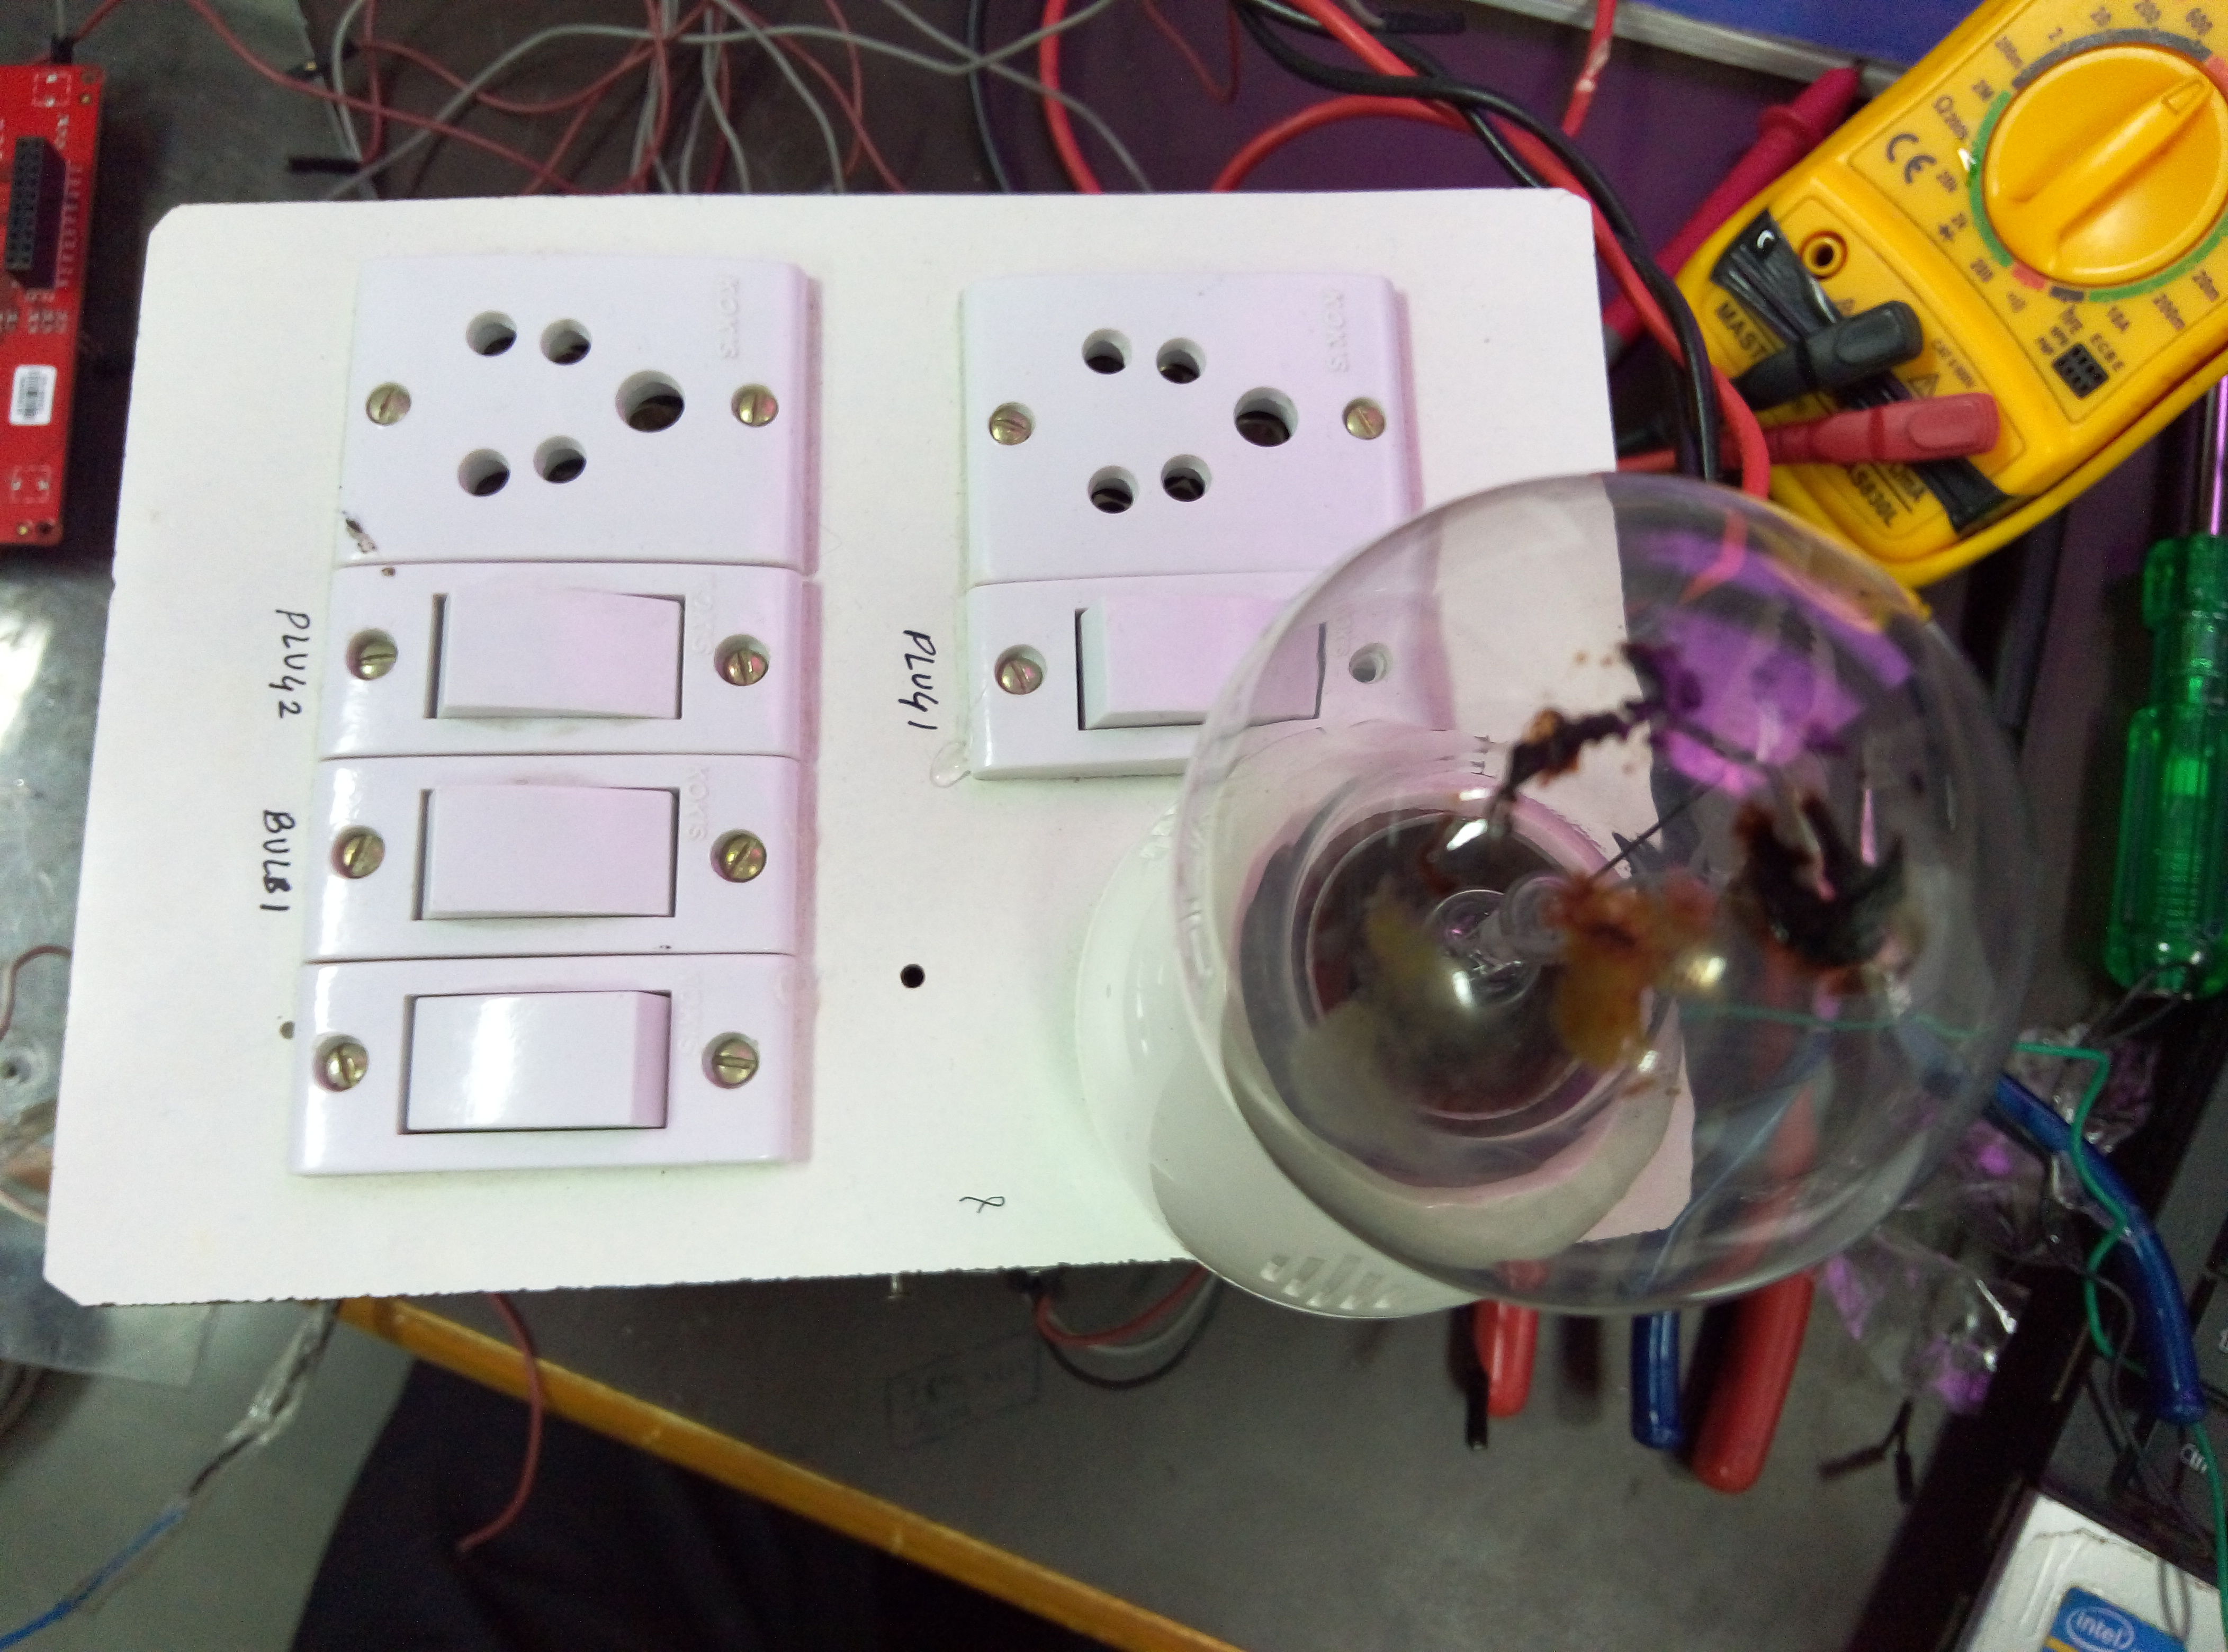
\includegraphics[width=300px]{plug1}
	\includegraphics[width=300px]{plug2}
\end{figure}
\newpage
\subsection*{Step 2}
Now assemble the $"measurement\ board"$ with the switch board at the location of your convenience. Make sure you have fixed the measurement board firmly with switch board as shown in figure below. 
\begin{figure}[h]
	\includegraphics[width=400px,height=200px]{assem1}
\end{figure}
\subsection*{Step 3}
Now connect and fix relay board with switch board at the location of your convenience as show in figure below
\begin{figure}[h]
	\includegraphics[width=400px,height=200px]{assem2}
\end{figure}
\newpage
\subsection*{Step 4}
Now connect the $CC3200-launchpad$ at the male headers 21 and 22. For more detail see board manual \autoref{100}
\begin{figure}[h]
	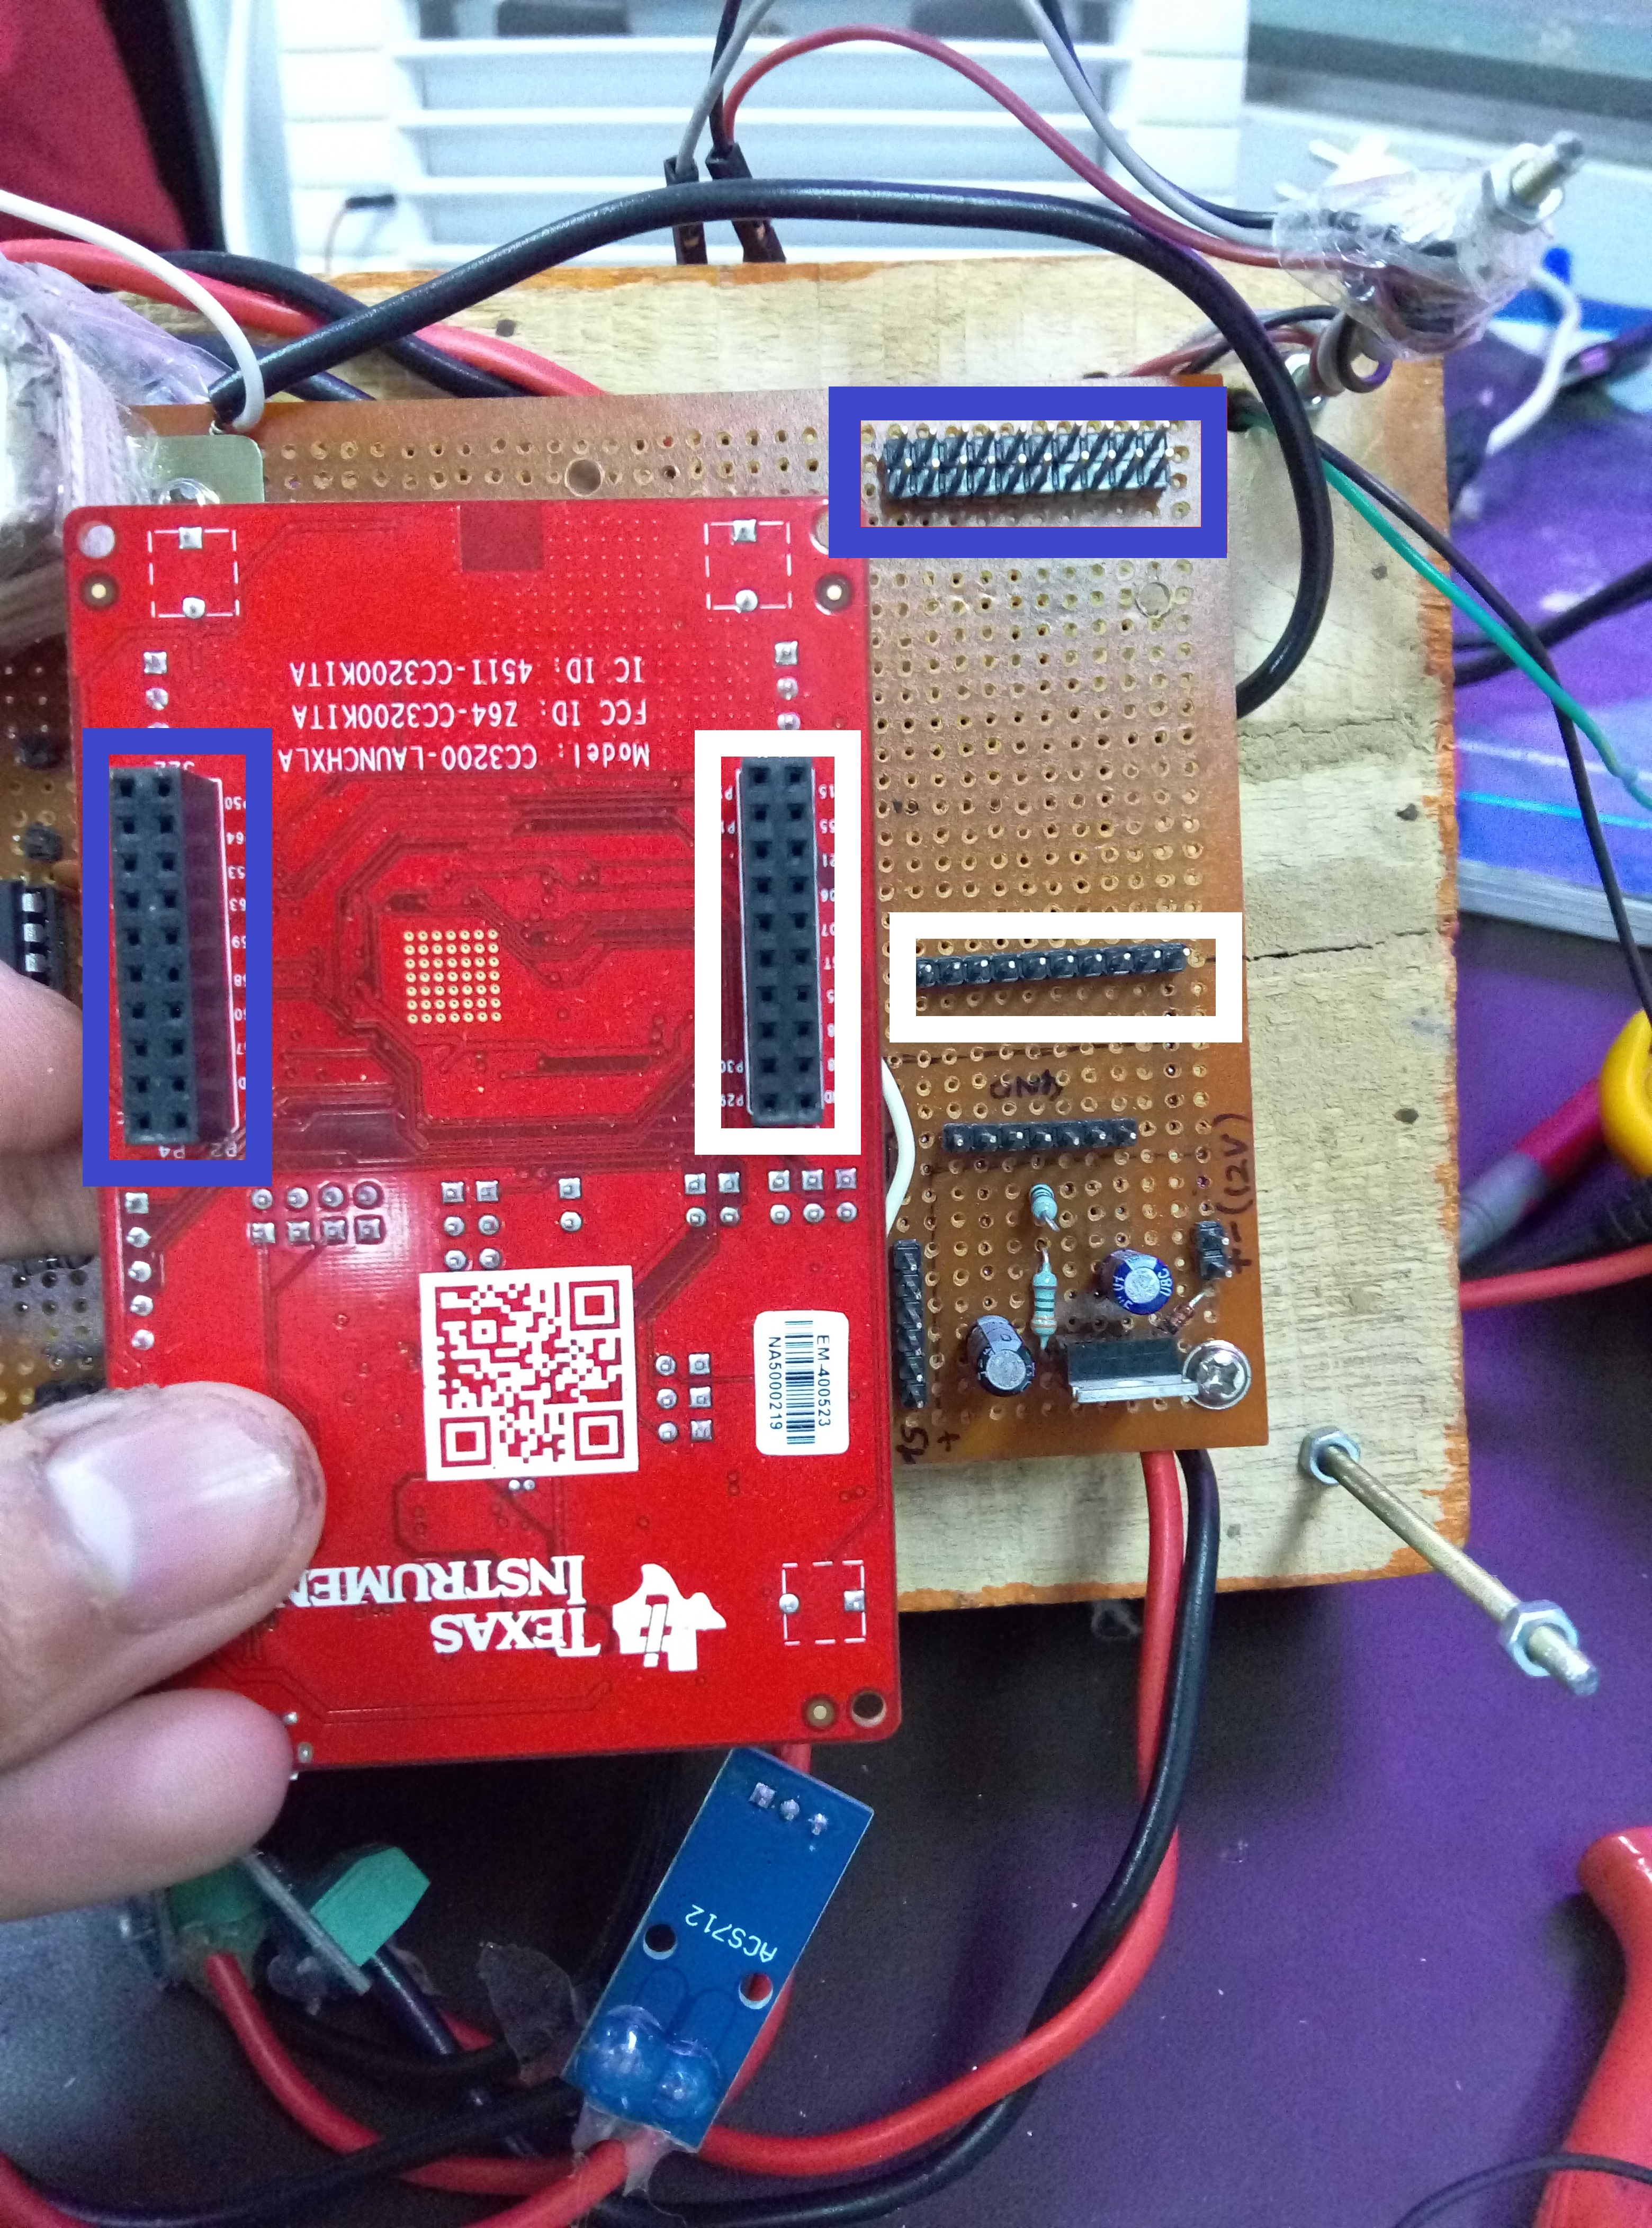
\includegraphics[width=300px,height=200px]{assem3}
\end{figure}
\subsection*{Step 5}
Now connect all the three hall sensor at pin number 1,2 and 3 appropriately on measurement board.for more detail see board manual \autoref{100}
\begin{figure}[h]
	\includegraphics[width=300px,height=200px]{assem4}
\end{figure}
\subsection*{Step 6}
Now connect $cc3200-launchpad$ and $Transformer$ with measurement board using female jumper as described below:
\begin{itemize}
	\item connect (pin1,pin4),(pin2,pin5) and (pin3,pin7) on the measurement board.
	\item connect pin7 and pin8 with the transformer output jumper.
	\item connect pin9 of measurement board to \textbf{$PIN59$} of cc3200 launchpad.
	\item connect pin17 of measurement board to \textbf{$PIN05$} of cc3200 launchpad.
	\item connect pin10 of measurement board to \textbf{$PIN58$} of cc3200 launchpad.
	\item connect pin12 of measurement board to \textbf{$PIN18$} of cc3200 launchpad.
	\item connect pin14 of measurement board to \textbf{$PIN60$} of cc3200 launchpad.
	\item connect pin15 of measurement board to \textbf{$PIN08$} of cc3200 launchpad.
	\item connect 5V and 3.3V pins of measurement board to $5V$ and $Vcc$ pins of cc3200 launchpad. 
	\item connect "Vcc" and "GND" of relay board with "5V" and "GND" of measurement board.
	\item connect the input pins of relay with $PIN64$, $PIN01$ and $PIN02$
	of CC3200 launchpad.
\end{itemize}
\newpage
\begin{figure}[h]
	\includegraphics[width=350px,height=350px]{assem5}
\end{figure}
for more detail about pin connection see board manual \autoref{100}
\subsection*{Step 7}
Now connect some more accessories to improve mechanical design and your \textbf{"Smart switch board"} is ready to use.

\newpage

\section{Software and Code}
\hspace{7mm} Code for web page is uploaded on github repo \href{https://github.com/eYSIP-2016/eYSIP2016-GHPowerMonitoring/tree/master/Softwares\%20and\%20Codes/Web\%20codes}{[Github link for Web page]}.\\

The wifi enabled device is designed in such a way, that it will POST a particular string in every 4 secs and reads the response from the server as shown in the figure \ref{29}. Note that exsisting system measures current and phase for 3 devices. Measurement for single phase supply voltage and frequency are shown as single reading.   

\begin{figure}[H]
	\centering
	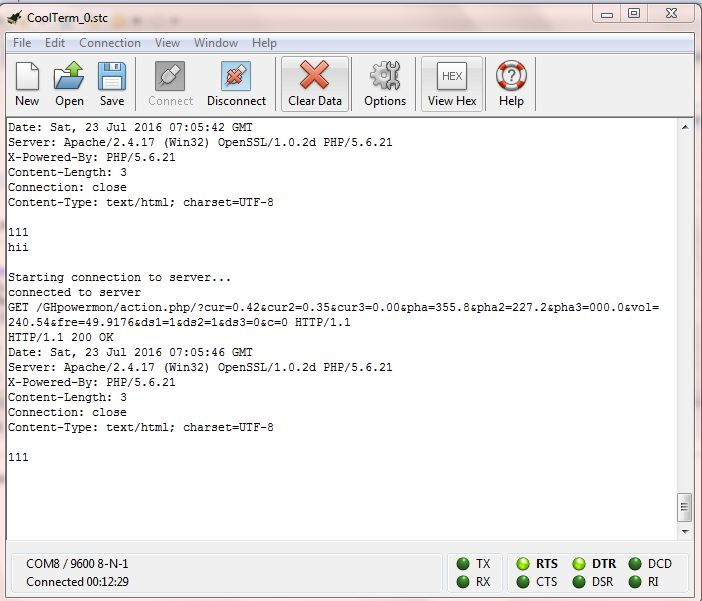
\includegraphics[width=15cm]{coolterm1.jpg}
	\caption{Sending Request after successful connection.}
	\label{29}
\end{figure}

\begin{itemize}
	\setlength\itemsep{0.2cm}
	
		\item{$action.php$ is the page accessed by the micro-controller, which in turn updates the database according to the data acquired.}
		\item{CC3200 uses queries to POST data and updates current values for devices 1,2,3 using $cur,cur2,cur3$, updates voltage using $vol$, frequency using $fre$,  phase of three devices using $pha,pha2,pha3$.}

	\item{logging the data}
	\begin{itemize}
		\item {$action.php$ is also capable of logging in database, it mainly  
			updates two tables in database.}
		\begin{itemize}
			\item {Table name - $reading$, It holds data under the columns $id$(Auto Increment), $Current1$, $Current2$, $Current3$, $Voltage$, $Frequency$, $Phase1$, $Phase2$, $Phase3 $, $reg\_date$ (Auto time stamp) }
			\begin{figure}[H]
				\centering
				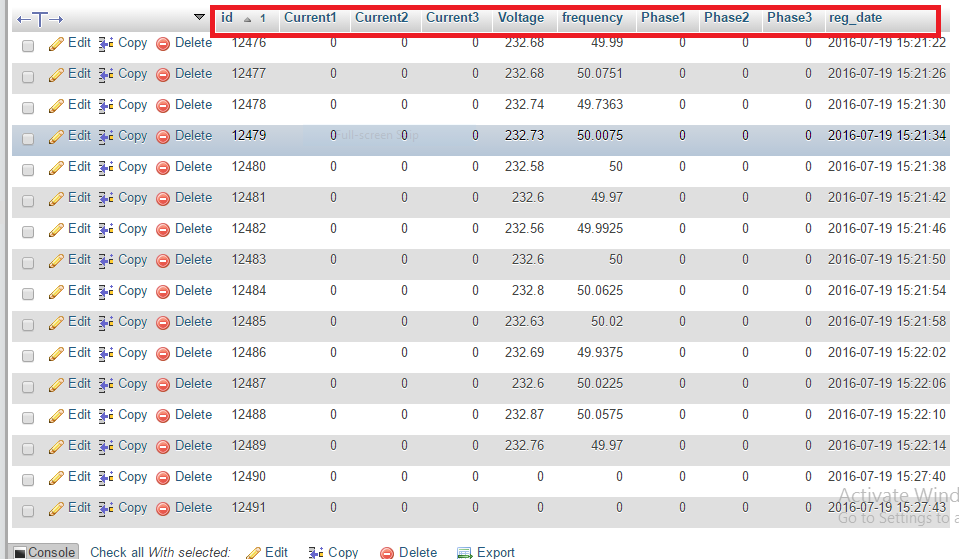
\includegraphics[width=15cm]{reading.png}
				\caption{Database table - $"reading"$}
				\label{1}
			\end{figure}
			
			\item{Table name - $para$, It only keeps the latest value under columns $RT$, infront of different row ids assigned to it. }
			
			\begin{figure}[H]
				\centering
				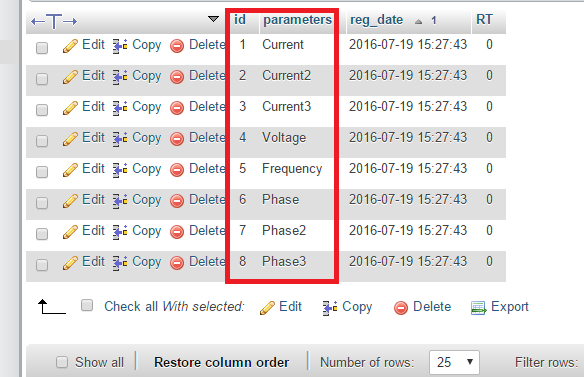
\includegraphics[width=15cm]{para.png}
				\caption{Database table - $"para"$}
				\label{2}
			\end{figure}
			
		\end{itemize}    
		\newpage	
	\end{itemize}
	\item{Real Time Plotting Graphs}
	\begin{itemize}
		\item{$current.html$ makes AJAX requests to $refresh.php$ which connects to database and updates it with latest data.}
		\item{With the latest data made available continuosly,Real Time updating graphs can be plotted.}
		\item{As the $chart.js$ will need data in JSON format, it requests to $action\_page.php$ to fulfill this requirement. }
	\end{itemize}
	\begin{figure}[H]
		\centering
		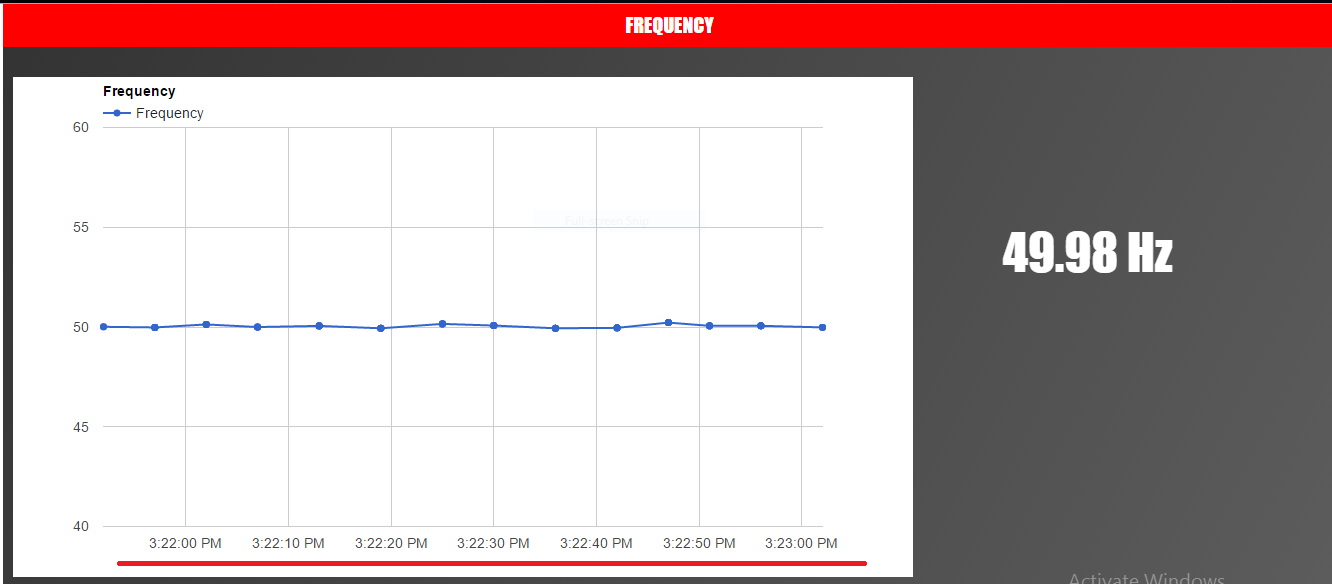
\includegraphics[width=15cm]{freq1.png} 
		\caption{Real Time Frequency plot 1 }
		\label{3}	
	\end{figure}
	Frequency is measured to be nearly 50Hz as shown in Figure \ref{3} and \ref{4} 
	\begin{figure}
		\centering
		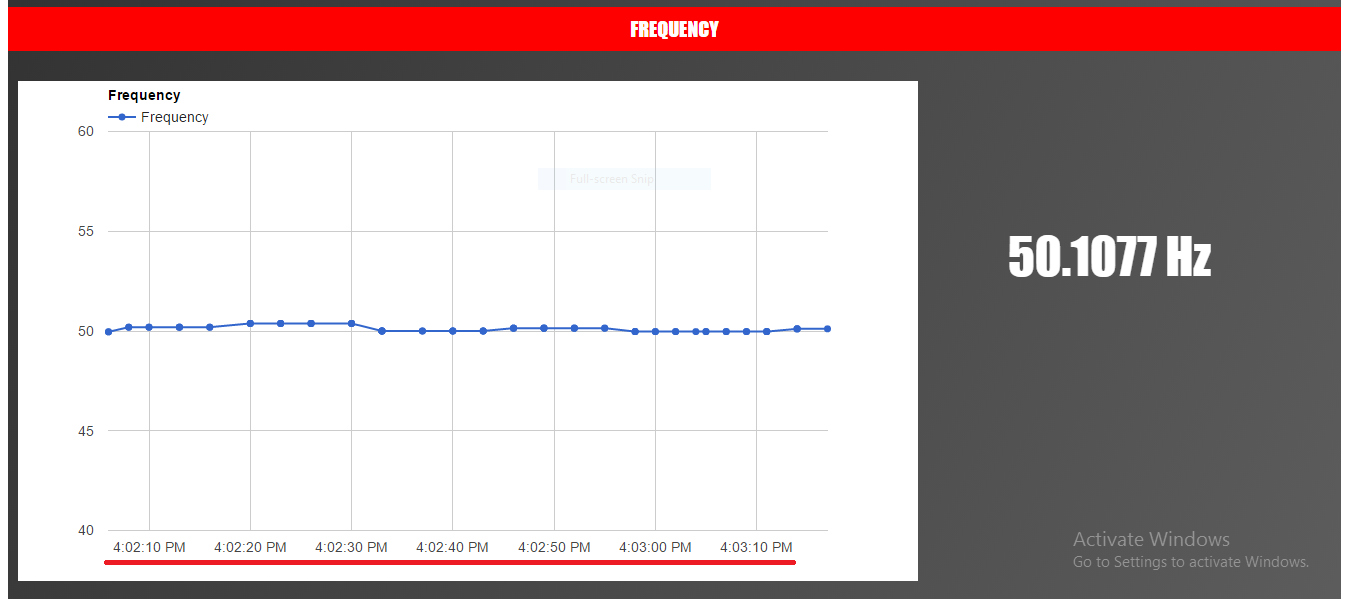
\includegraphics[width=15cm]{freq_mov.png}
		\caption{Real Time Frequency plot 2 }	
		\label{4}
	\end{figure}
	\newpage
	\item{Plotting the logged data }
	\begin{itemize}	
		\item{The logged data is gathered and converted into JSON by $action\_graph\_week.php$. \\ 
		Note that dip in voltage and frequency plot is due to action of switching on/off the device for testing purpose. Also the graph shows plot for 1 hour device operation.}
		\begin{figure}
			\centering
			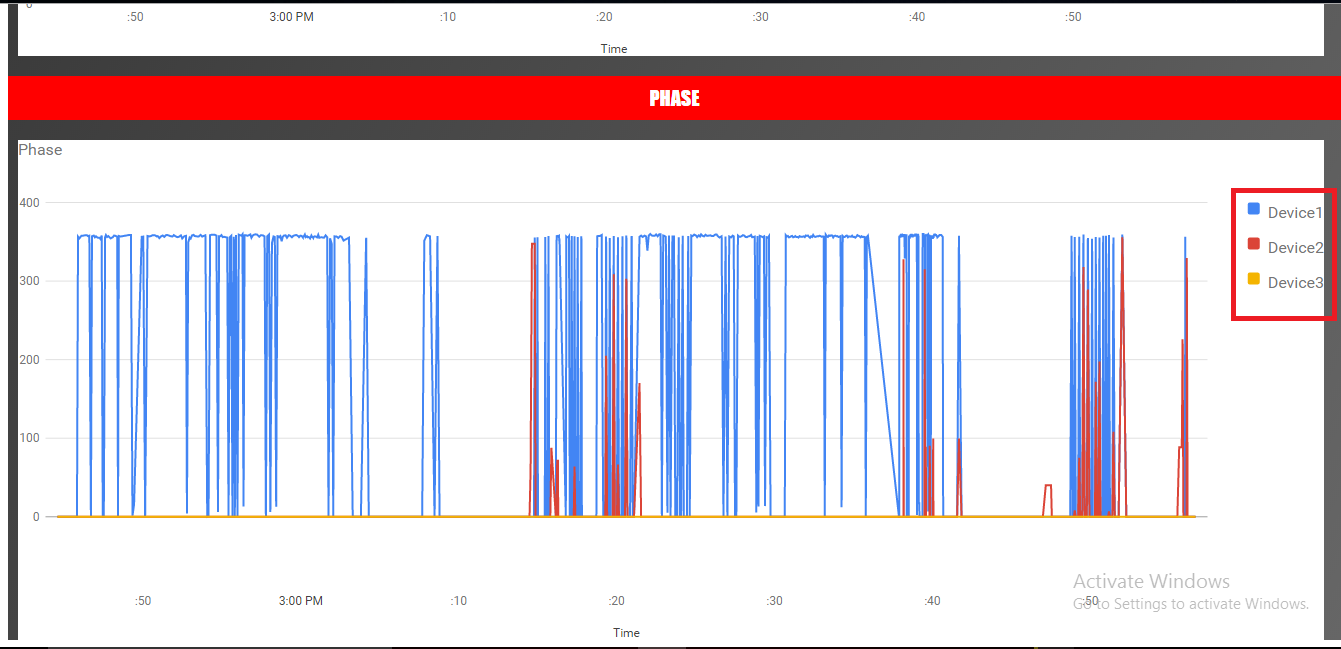
\includegraphics[width=15cm]{phase_today.png}
			\caption{Logged Phase data}
			\label{5}
		\end{figure}
		\item Oscillation in phase is due to reason that phase difference for resistive load is zero and on circular plot 0 and 360 are overlapping but on linear scale plot it appears to oscillate.
		\begin{figure}
			\centering
			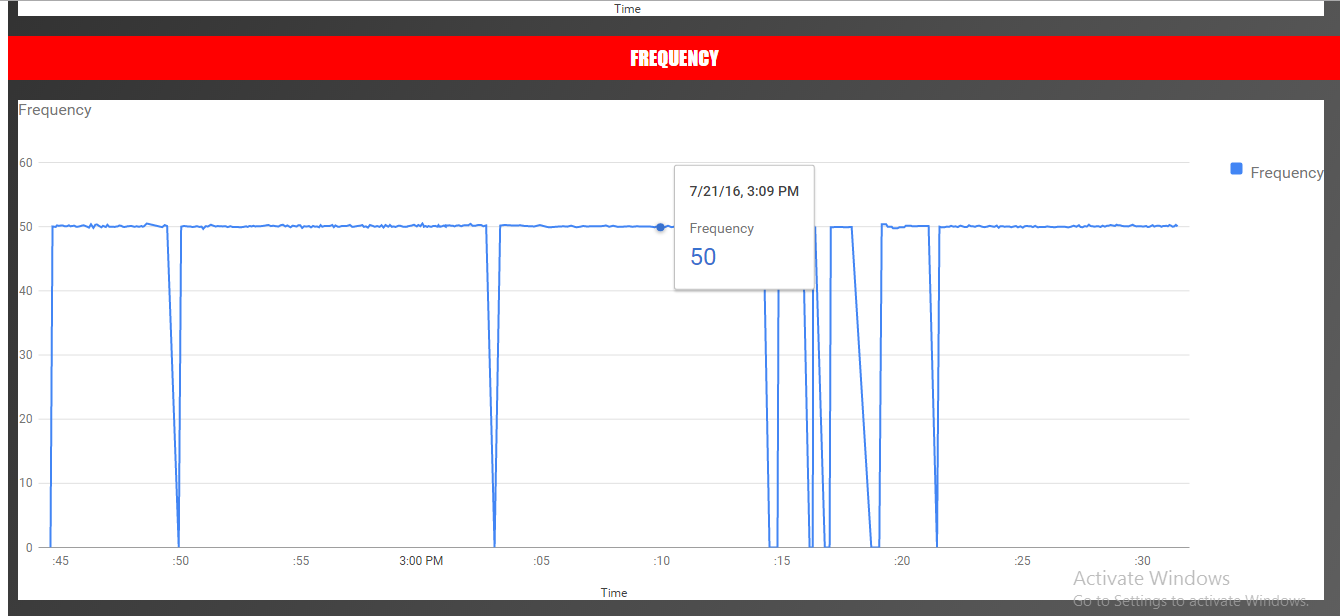
\includegraphics[width=15cm]{frequency_today.png}
			\caption{Logged Frequency Data}
			\label{6}
		\end{figure}
		
		
		
		\begin{figure}[H]  \centering
			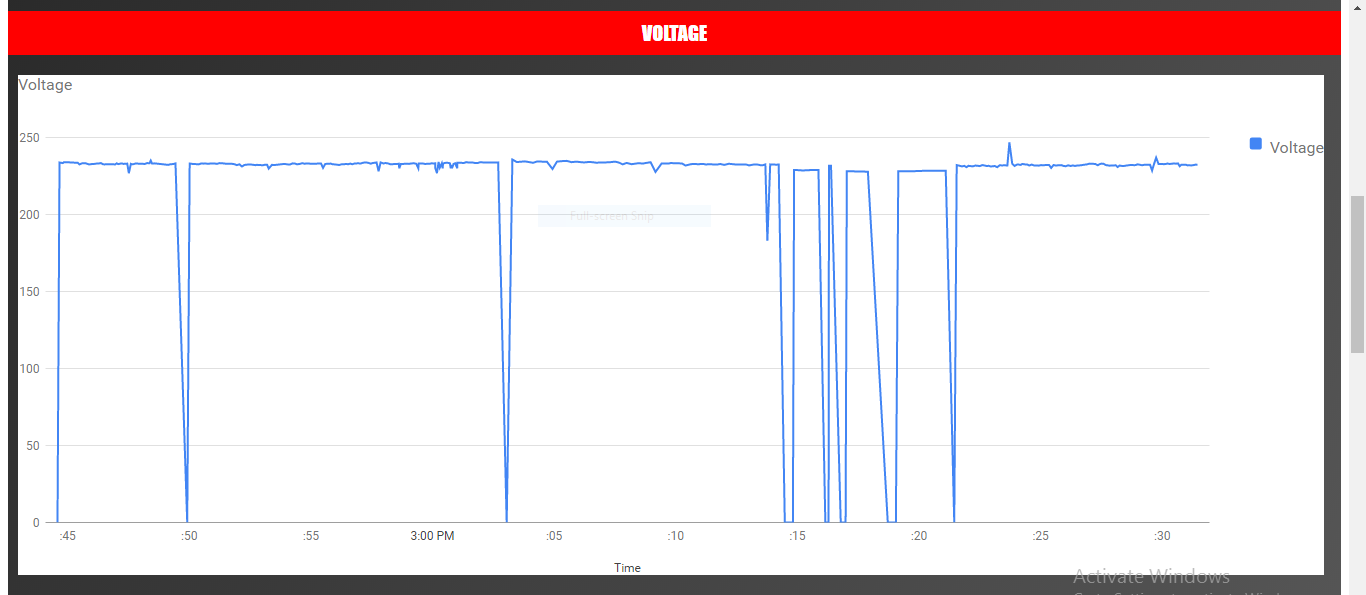
\includegraphics[width=14cm]{voltage_today.png}
			\caption{Logged Voltage Data}
			\label{7}
		\end{figure}
		
		
		
		\begin{figure}[H]  \centering
			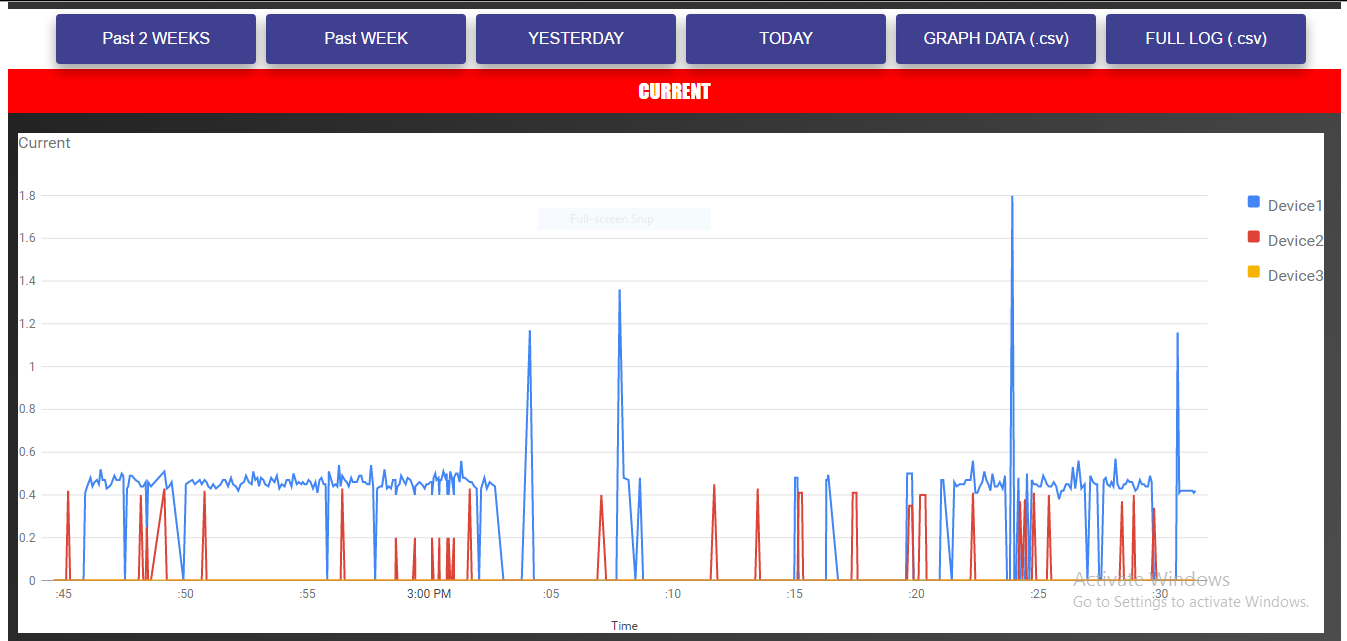
\includegraphics[width=15cm]{current_today.png}
			\caption{Logged Current Data}
			\label{8}
		\end{figure}
		
		
		
		\item{The graph is plotted by $stable\_chart\_loop.js$ which creates a graph according to datatable generated after user selected a particular period.}
		
		
		\begin{figure}[H]  \centering
			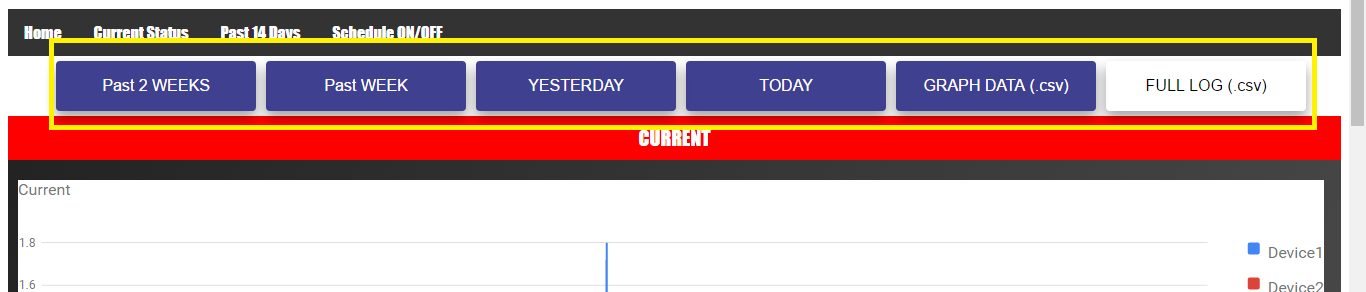
\includegraphics[width=15cm]{selection_buttons.png}
			\caption{Selection Buttons}
			\label{9}
		\end{figure}
		
		\item{As shown in above image, user can select the period ,which will then accordingly request and generate JSON data required for $stable\_chart\_loop.js$ }
		
		\item{The graph can be selectively highlighted and observed with timestamp and value on tool-tip.}
		
		\hspace{10px}
		
		\begin{figure}[H]  \centering
			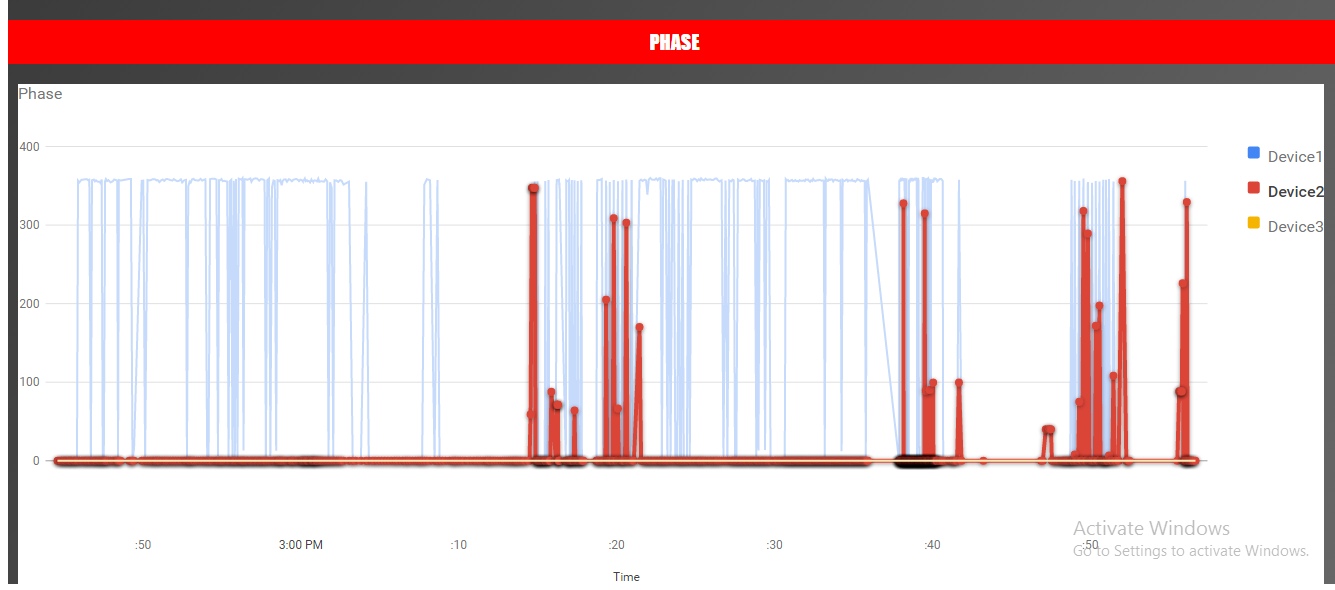
\includegraphics[width=15cm]{selectively_graph.png}
			\label{10}
			\caption{ Selective view of graphs for multiple devices.} 
		\end{figure}
		
		\hspace{10px}
		
	\end{itemize}
	\item{Feedback System}
	\begin{itemize}	
		\item{In request url cc3200 also provides feedback using $ds1,ds2,ds3$. Figure \ref{29} shows the request url.}
		\item{In response server will update it with a boolean sequence for eg.$100,110,000...$ indicating switch status for each one of the 3 devices  } 
		\item{Then the server waits for feedback in next request, which are provided by cc3200 in variables $ds1,ds2,ds3$}
		
		
		\begin{figure}[H]  \centering
			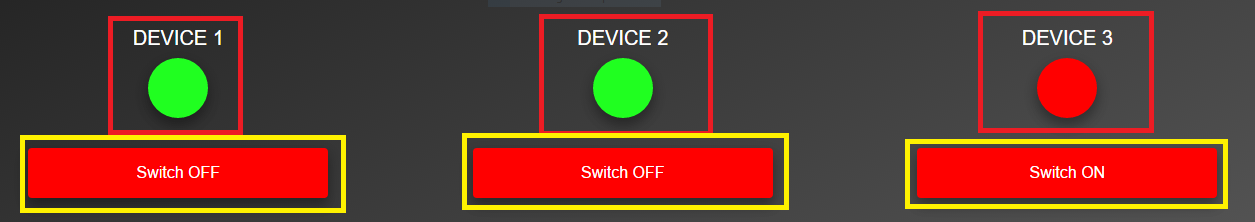
\includegraphics[width=15cm]{feedback.png}
			\caption{Feedback system}
			\label{fig: figure_feedback}
		\end{figure}
		\hspace{10px}
		\item{Figure \ref{fig: figure_feedback} shows circular blocks which shows current device status obtained in request.\\ If  a device is showing OFF when it should be ON or showing ON when it should be OFF, then system fault can be detected. It indicates that maybe there is no device or it is not functioning properly. }
	\end{itemize}
	\item{Scheduling and Control}
	\begin{itemize}	
		\item{The scheduling page allows user to schedule ON and OFF (as Radio buttons)  and selection 'FROM' time and 'TO' time using input text field and datetimepicker.}
		\hspace{10px}
		
		\begin{figure}[H]  \centering
			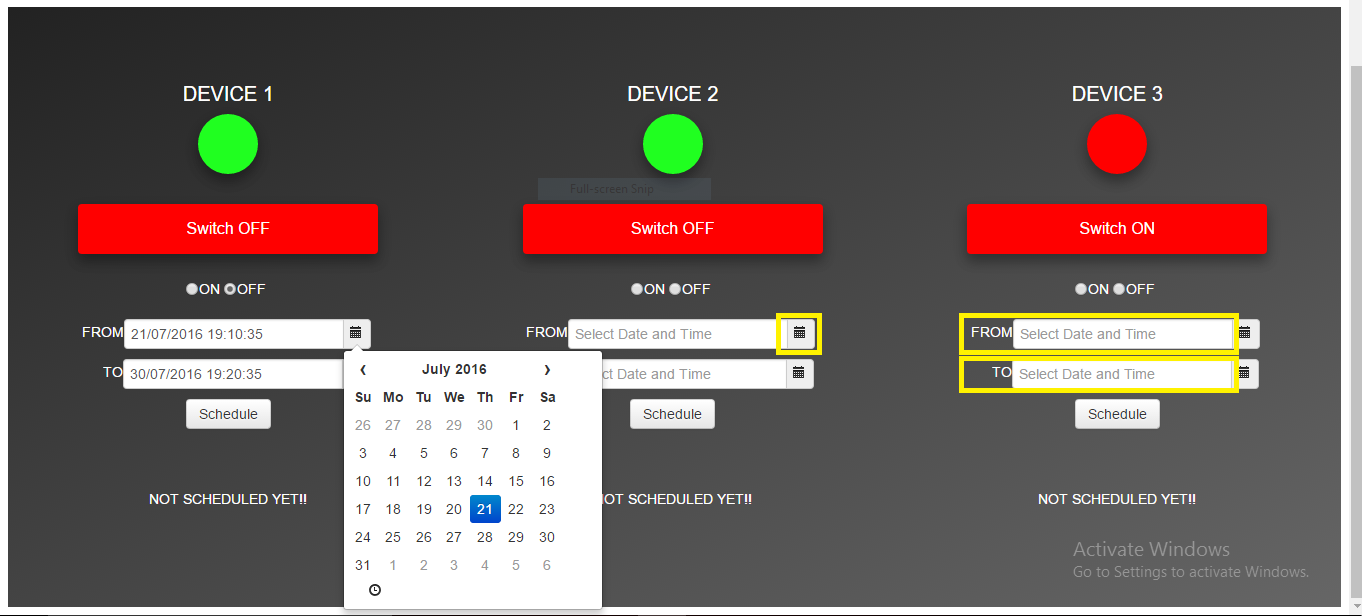
\includegraphics[width=15cm]{scheduler.png}
			\caption{ ON/OFF Scheduler}
			\label{17}
		\end{figure}
		
		\item{The Scheduling datetime is submitted to $selection.php$ which update values in database, which are then further compared with every timestamp and a boolean string response for connected devices.}
		
		\begin{figure}[H]  \centering
			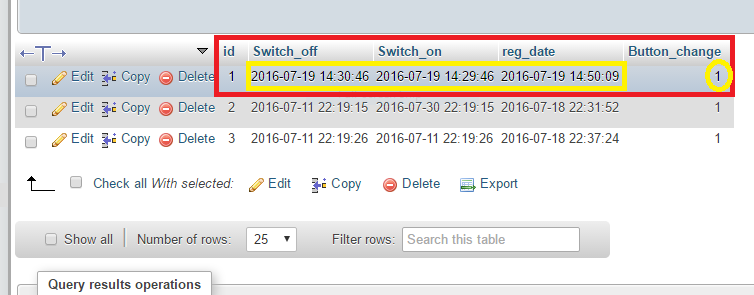
\includegraphics[width=15cm]{scheduled.png}
			\caption{ Database Table $scheduled$ - if not scheduled }
			\label{18}
		\end{figure}
		\item{As shown in Figure \ref{18} If initial status of $button\_change$ is 1, it means scheduling is inactive.}
		\begin{figure}[H]  \centering
			\includegraphics[width=15cm]{scheduled_table.png}
			\caption{ Database Table $scheduled$ - if scheduled }
			\label{19}
		\end{figure}
		
		\item{Initial status of $button\_change$ is 0, with updated values of $Switch\_on$ time and $Switch\_off$ time(Scheduled values on left frame for reference).}
		
		\item{As $Switch\_off$ Time is smaller than $Switch\_on$ time, the Scheduler will automatically Switch OFF the device and wait for next Switch ON command.}
		
		\item{Buttons are available for all three devices, which have the capability to switch devices off/on.}
		
		
		\begin{figure}[H]  \centering
			\includegraphics[width=13cm]{power.png}
			\caption{ Database table $"Power"$}
			\label{20}
		\end{figure}
		
		\item{Figure \ref{20} shows that First button's data is submitted to $button\_status.php$, Similarly for second button's data is submitted to $button\_status2.php$,and same goes for third button $button\_status3.php$.\\The $ Choice $ column stores the last selected choice in log selection buttons. }
		
	\end{itemize}
\end{itemize}	
\newpage
\section{Use and Demo}
\begin{itemize}
	\item{Configure the Smart Switch-board using Serial Terminal software}
	
	\begin{figure}[H]  \centering
		\includegraphics[width=13cm]{coolterm2.jpg}
		\caption{Interactive Interface - Initial Options}
		\label{34}
		
		\includegraphics[width=13cm]{coolterm3.jpg}
		\caption{Select an option by entering an Integer value.}
		\label{30}
	\end{figure}
	\begin{figure}[H]  \centering
		\includegraphics[width=13cm]{coolterm4.jpg}
		\caption{Enter Wi-Fi SSID and Password}
		\label{31}
	\end{figure}
	\begin{figure}[H]  \centering
		\includegraphics[width=13cm]{coolterm5.jpg}
		\caption{Return to Main Menu}
		\label{32}
	\end{figure}    	
	\begin{figure}[H]  \centering
		\includegraphics[width=13cm]{coolterm6.jpg}
		\caption{Sign Out}
		\label{33}
		
	\end{figure}
	
	\item{Open the webpage. (NOTE: The Web Site was developed and tested on a localhost)}
	
	
	\begin{figure}[H]  \centering
		\includegraphics[width=15cm]{homephp.png}
		\caption{Home Page}
		\label{21}
	\end{figure}
	
	
	\item{Figure \ref{21} shows the home page of the web based GUI, with 3 buttons viz. \textit{Start Monitoring, Get Log Data and Schedule Event}.}
	\item{ Under the title of page, a navigation bar is present. Navigation bar will help user navigate between pages.}
	
	\item{Next is the current status page.See \autoref{27}.\\ The first Division shows the current(in A) flowing in the 3 devices. \\BLUE for Device 1\\RED for device 2\\YELLOW for device 3 }
	
	\begin{figure}[!h]%
		\centering
		\subfloat[]{{\includegraphics[width=6cm]{Live_data} }}%
		\qquad
		\subfloat[]{{\includegraphics[width=6cm]{Live_data2} }}%
		\caption{Real time updating graph with different stamp }%
		\label{27}%
	\end{figure}
	
	\item{Divisions for voltage(in V)and frequency(in Hz) follow Current's division.	
		\\ Only one line chart is being made for these two parameters as they are same for all three devices.}
	
	\item{Last division represents phase difference(in deg) of the three connected devices. See  \autoref{27} for reference .\\BLUE for device 1\\RED for device 2\\YELLOW for device 3 } 
	
	\begin{figure}[H]
		\centering
		\includegraphics[width=15cm]{logging_page.png}
		\caption{Logging page}
		\label{24}
	\end{figure}
	
	
	\item{\autoref{24} shows the logging page.}
	\item{As shown in the \autoref{24} the first four buttons provided are for period selection, and the last two are download links for .csv format for graph data and complete log data respectively.   }
	
	\item{By clicking any of the four buttons, graph will be plotted for the given period, and $Graph\ Data$ download link will generate a log for that specific period in .csv format as shown in \autoref{22}.}
	
	\begin{figure}[H]  \centering
		\includegraphics[width=15cm]{log.png}
		\caption{Graph Data Log}
		\label{22}
	\end{figure}
	%*************************************************************************
	\item{$Today$ button will generate graph with Only That day's data.\\$Yesterday$ button will generate graph for previous data only.\\
		$Past\ week$ will generate filtered hourly data in the past week.\\
		$ Past\ 2\ Weeks$  will generate filtered hourly data in the past 2 weeks.\\ These are defined in $action\_graph\_week.php$.}
	
	
	%-------------------------------------------------------------------------- 
	
	\item{Full log in .csv format is always available for the user to download .}
	
	\begin{figure}[H]  \centering
		\includegraphics[width=15cm]{full.png}
		\caption{Full Log}
		\label{26}
	\end{figure}
	%***********************************************************************
	\item{ The last page is $Schedule\ ON/OFF$ page. This is the controlling page with features like scheduling and switching ON/OFF.\\ 
	The button highlighted in \autoref{fig: button} is the switch.\\It can be noted that the text on it changes according to current button status and circular block which indicates the actual device status.\\
	GREEN represents ON status.\\RED represents OFF status.
	
	\item{Just below every switch button there is a scheduler which can schedule ON/OFF. Scheduler is shown in \autoref{35}}\\
			
			\begin{figure}[H]  \centering
				\includegraphics[width=15cm]{feedback.png}				\caption{Button}
				\label{fig: button}
			\end{figure}

			\begin{figure}[H]  \centering
				\includegraphics[width=15cm]{scheduler.png}
				\caption{Control page}
				\label{35}
			\end{figure}					

		The user first have to make a choice between ON/OFF radio buttons.If no selection is made it will be automatically counted as OFF . }
	\item{ Then the user have to fill the two input fields namely $FROM$ and $TO$ as per requirement.See \autoref{35}}
	\item{Scheduled Time-interval and Type will be notified as text.See \autoref{35}}
	
	%-------------------------------------------------------------------------
	
	-
\end{itemize}
\newpage
\section{Future Work}
\begin{itemize}
	\item{Current Web GUI is not responsive and will not work properly on mobile phones. Using Bootstrap (HTML,CSS framework) site can be made responsive.}
	\item{Zoom Function can be added in charts for better user experience.}
	\item{Features to control frequent or repeated Scheduling can be added.}
	\item {Support for more devices can be added even when monitoring is available for few devices due to limited ADCs.}
	\item{Circuit can be miniaturized by designing measurement board on PCB and using Redbear Wifi-mini or cc3200 micro, which can increase portability}
	\item{Phase measurement accuracy can be improved.}
	
\end{itemize}
\newpage
\section{Bug report and Challenges}
\subsection*{Bug report}
\begin{itemize}
	\item For accurate measurement of phase please calculate the phase difference created by coupling capacitor applied to current wave for removing offset voltage.
	\item Use \textbf{TI-RTOS} \& \textbf{Free-RTOS} for fast processing and transient analysis of the electrical parameters.
	\item{SQL Injection - A code injection technique, used to attack data-driven applications, in which nefarious SQL statements are inserted into an entry field for execution. Blacklisting some characters can prevent attacks.For more details refer \href{www.w3schools.com/sql/sql_injection.asp}{W3schools SQL injection} }
	\item{Lightweight protocols Like MQTT can be used for better performance.}
	\item{Security can be improved by adding Cryptography techniques like AES.}
\end{itemize}
\subsection*{Challenges}
\begin{itemize}
	\item To add header files to the code composer studio project right click on project ,go to properties than select linked resources and than add $CC3200\_sdk$. After adding sdk to linked resources than again right click on project, go to GNU compiler and include directories to it.
	\item The debug mode of CCS load the program into RAM of CC3200 launchpad so to load program into ROM use \textbf{Uniflash}.
	\item Before loading the program into flash please follow the below procedure
	\begin{itemize}
		\item Format the whole CC3200 launchpad's ROM using \textbf{format} tab.
		\item Load \textbf{service pack}, which is compatible with your launchpad's version.
		\item Now load the .bin file of project. 
	\end{itemize} 
	\item For loading program into ROM select \textbf{mcu.bin} tab in Uniflash and than add the .bin file of the project.After adding the .bin file program MCU using program tab.
	\item To write program for CC3200-launchpad please take help from \textbf{Driverlib API's},\textbf{Simplelink API's} and all the API module files present inside CC3200sdk folder.For more details \href{https://github.com/eYSIP-2016/eYSIP2016-GHPowerMonitoring/tree/master/Documents/CC3200\%20doc}{Documents inside Github repo }
	   
\end{itemize}

\begin{thebibliography}{li}
		\item{Stack Overflow  \href{www.stackoverflow.com}{www.stackoverflow.com}}
		\item{TutorialsPoint  \href{tutorialspoint.com/}{www.tutorialspoint.com/}}
		\item{GitHub  \href{github.com}{www.github.com}}
		\item{W3Schools  \href{http://www.w3schools.com/}{www.w3schools.com/}}
		\item{TI E2E Community \href{TI E2E Community}{	https://e2e.ti.com/}}
		\item{Instructables \href{www.Instructables .com}{www.instructables.com}}
		\item\href{https://github.com/eYSIP-2016/eYSIP2016-GHPowerMonitoring/tree/master/Documents}{Driver Library and Simplelink Library}{\label{50}}
		
\end{thebibliography}

\begin{appendices}
\chapter{Measurement board manual}
\label{100}
\section{Abstract}
\hspace{7mm} The measurement board is an analog front end, which is used to manipulate the input signal according to the MCU unit. The signals generated by this board will be processed by MCU in the further sections of hardware. Basically this board provides a common platform where microcontroller unit can be able understand the actual electrical signal. This measurement board has a set of small circuits such as zero crossing detector, buffers, voltage dividers and filters etc.  

\newpage
\section{Circuit diagram}
\begin{figure}[h]
	\includegraphics[width=380px,height=380px]{schematic}
\end{figure}
\newpage
\section{Description of circuit diagram}
\label{89}
\begin{enumerate}
	\item \textbf{Power block:}\\
	This circuit block is based on 7805 (5V regulator IC). It has a 10uF electrostatic capacitor at input side. A 10 ohm resistor is used at the ground terminal of voltage regulator to protect it by limiting its output current.A first order low pass circuit is applied at output side to remove ripple present in output voltage.
	\begin{figure}[h]
		\includegraphics[width=380px,height=380px]{powerblock}
	\end{figure}
	\item \textbf{Hall sensor block:}\\
	This circuit block is used to convert the current wave of all the three electrical appliances into a proportional voltage wave used for the measurement. Three coupling capacitor is applied to remove DC offset voltage which is coming because of Hall sensor module for detailed explanation go through data sheet of ACS712 \href{./datasheet/ACS712-Datasheet.pdf}{Datasheet}. Three 10K ohm resistor are applied to change the output impedance of the circuit.
	\begin{figure}[h]
		\includegraphics[width=380px,height=380px]{hallblock}
	\end{figure}
	\item \textbf{Transformer block:}\\
	This circuit block is used to step down and manipulate the voltage wave according to reference voltage (1.467V) of CC3200 launchpad. For this purpose a high impedance voltage divider circuit is applied to step down the voltage by 10:1. We choose to apply high impedance voltage divider to decrease loading effect and power loss. A 0.01uF ceramic cap is applied at the output side to provide pickup to the ADC channel of cc3200 MCU. For detailed explanation please go through \href{http://processors.wiki.ti.com/index.php/CC32xx_ADC_Appnote}{ADC Appnote cc32xx}. Two 1M ohm resistor is applied to eliminate attenuation coming in rectified voltage wave.
	\begin{figure}[h]
		\includegraphics[width=380px,height=380px]{transblock}
	\end{figure}
	\item \textbf{Zero crossing detector block:}\\
	This circuit block is used to generate a pulse whenever the AC signal crosses the zero level. This circuit is basically a comparator followed by first order RC circuit. Output is taken across the resistor. The logic behind this circuit is that whenever the input wave crosses the zero level the comparator output will either go from 5V to 0V or from 0V to 5V, so we can consider this phenomena as switching of first order RC circuit. During transient, output voltage expression across the resistor is \autoref{96}. The time constant ($\tau$) of circuit is used to determine the width of pulse.\\
	\hspace{1cm}This circuit is used four times in the measurement board for generating phase and frequency signals. A high speed diode is applied at output side to remove negative pulse. High speed diode is used because it has less amplitude reverse recovery current, so the circuit output doesn't have unusual pulses.
	\begin{figure}[h]
		\includegraphics[width=380px,height=380px]{zcdblock}
	\end{figure}
	\item \textbf{Buffer block:} \\
	This block is used to clip the current wave and manipulate it according to the ADC channel of CC3200 MCU. Buffer is also used to protect the ADC channel from electrostatic surge by isolating it from the electrolytic coupling capacitor. This block is used three times to generate three current signal.
	\begin{figure}[h]
		\includegraphics[width=380px,height=380px]{bufferblock}
	\end{figure}
	  
\end{enumerate}
\section{DIY}
Here we are including a special feature in the manual. By reading the manual now you can make this board by your self. To make it your self please follow the following instruction:
\subsection*{List of components}
\begin{tabular}{|l|c|c|}
	\hline
	\textbf{Name of component} & \textbf{Specification}& \textbf{Quantity}\\ \hline
	Resistor& 10 ohm (1/4W)&1\\ \hline
	&330 ohm (1/4 W)&1 \\ \cline{2-3}
	&1K ohm (1/4W)&3 \\ \cline{2-3}
	&10K ohm (1/4W)&3 \\ \cline{2-3}
	&33K ohm (1/4W)&4 \\ \cline{2-3}
	&100K ohm (1/4W)&5 \\ \cline{2-3}
	&900K ohm (1/4W)&1 \\ \cline{2-3}
	&1M ohm (1/4W)&2 \\ \hline
	Electrostatic Capacitor& 0.1uF (50V)&1\\ \cline{2-3}
	&0.22uF (10V)&3 \\ \cline{2-3}
	&10uF (50V)&1 \\ \hline
	Ceramic capacitor& 0.01uF (103)&8 \\\hline
	Diode&IN4148 (high speed diode)&4 \\\hline
	Operational& LM324&2\\
	Amplifier&\textit{Quard opamp IC}&\\\hline
	Rectifier&DB-107&1 \\\hline
	Berg strip&Male(40x1)&2 \\\cline{2-3}
	&Female(40x1)&1\\\hline
	Breadboard \& Wires & -&1 \\\hline
	Soldering iron and wire& 40W&1 \\\hline
	General purpose PCB & 15cmx15cm&1 \\\hline	
\end{tabular}
\\\\\\\\
\subsection*{Procedure}
\begin{itemize}
	\item Before starting to build the circuit make sure you have gone through the circuit description and understand the circuit completely.
	\newpage
	\item Collect all the component, listed above if you are not able to find them than you may apply components of approximate value.\\
	\begin{center}
		\includegraphics[width=300px]{diy1}
	\end{center}
	\item First of all check the circuit on the breadboard whether it is working or not, After that u can solder the circuit on PCB board. We recommend you to use IC holders for mounting IC, because soldering temperature may damage the IC. 
	\begin{center}
		\includegraphics[width=300px]{diy2}
	\end{center}
	\item Start making small circuit block on different the part of PCB as explained in the description of circuit diagram. for more details \autoref{89}.
	\begin{center}
		\includegraphics[width=200px,angle=-90]{diy3}
	\end{center}
	\begin{center}
		\includegraphics[width=350px,angle=180]{diy4}
	\end{center}
	\item When small section of circuit schematic got soldered on PCB than start connecting those small section according to label provided in schematic.
	\item After connecting all the circuit blocks please double check your circuit using multimeter connection check, whether there is any short circuit or not. 
	\item Cheers!!! your measurement board is ready to use, now you can connect CC3200 launchpad to it and start software part. 
\end{itemize}
\section*{Pin Description}
\begin{center}
	\includegraphics[width=350px,height=400px]{board}
\end{center}
\begin{itemize}
	\item \textbf{PIN 1:} Hall sensor 1 input pin 
	\item \textbf{PIN 2:} Hall sensor 2 input pin
	\item \textbf{PIN 3:} Hall sensor 3 input pin
	\item \textbf{PIN 4:} DC blocked current signal 1
	\item \textbf{PIN 5:} DC blocked current signal 2
	\item \textbf{PIN 6:} DC blocked current signal 3
	\item \textbf{PIN 7 \& PIN 8:} Transformer(230V/9V) output pins
	\item \textbf{PIN 9:} processed voltage signal that will going into ADC pin
	\item \textbf{PIN 10:} processed current signal that will going into ADC pin
	\item \textbf{PIN 12:} Phase 1 signal 
	\item \textbf{PIN 14:} processed current signal that will going into ADC pin
	\item \textbf{PIN 15:} Phase 2 signal 
	\item \textbf{PIN 16:} processed current signal that will going into ADC pin
	\item \textbf{PIN 13:} Phase 3 signal 
	\item \textbf{PIN 17:} Frequency signal
	\item \textbf{PIN 18:} 5V header pins
	\item \textbf{PIN 19:} Vcc header pins
	\item \textbf{PIN 20:} Gnd header pins
	\item \textbf{PIN 21 \& PIN22:} Headers for mounting of CC3200 launchpad
\end{itemize}
\newpage
\section{Circuit output the each pin}
\subsection*{At Pin number 1,2 \& 3}
At these pins current wave with 2.5V offset will appear. The offset is because of hall sensor module used for current sensing unit.\\
for further details go through datasheet of ACS712 module \href{./datasheet/ACS712-Datasheet.pdf}{Datasheet}
	\begin{center}
		\textbf{OUT = $2.5 + asin(wt)$}
	\end{center}
	\begin{flushleft}
		\textbf{Where:}\\
			a = amplitude of $sin$ wave in V.\\
			$w$ = angular frequency of current signal in (rad/sec).\\
			t = time in sec.\\
	\end{flushleft}
	
\subsection*{At Pin number 4,5 \& 6}
At these pins current wave without offset will appear.\\
\begin{center}
	\textbf{OUT = $asin(wt)$}
\end{center}
\begin{flushleft}
	\textbf{Where:}\\
	a = amplitude of $sin$ wave in V.\\
	$w$ = angular frequency of current signal in (rad/sec).\\
	t = time in sec.\\
\end{flushleft}

\subsection*{At Pin number 12,13,15 \& 17}
At these pins output of zero crossing circuit will appear.\\
\begin{center}
	\label{96}
	%\textbf{OUT = $5e^-^(^t^/^\u^)$}
	\textbf{$OUT = 5e^{-t/\tau}$}
\end{center}
\begin{flushleft}
	\textbf{Where:}\\
	$\tau$ = time constant of zero crossing detector circuit.\\
	t = time in sec.\\
\end{flushleft}
\subsection*{At Pin number 9,10,14 \& 16}
Voltage and current signal manipulated according to reference voltage of CC3200 launchpad \\

\subsection*{At Pin number 18,19 \& 20}
5V, Vcc and ground pins on the measurement board.  \\
\subsection*{At Pin number 21 \& 22}
Headers for connecting CC3200-launchpad. \\
\end{appendices}
\end{document}

